% !TEX program = latexmk
% !TEX encoding = UTF-8 Unicode
% XJTU submission preview lane generated from thesis/cn on 2026-05-10.
% This is not an official submission PDF until metadata and 2025+ university requirements are confirmed.

\documentclass[
    master,
    % blind,
    % plgck,
]{XJTU-thesis}

\title{有机光电存算一体系统的算法—器件协同设计研究}{Algorithm--Device Co-design for Organic Optoelectronic Compute-in-Memory Systems}
\degree[A]{硕士}{Master of Science}
\author{李松桥}{Songqiao Li}
\advisor{导师待确认}{职称待确认}{Advisor To Be Confirmed}{Title TBD}
\subject{材料科学与工程}{Materials Science and Engineering}
\submitdate[2026][05]

% Defense/reviewer metadata placeholders. Replace before any formal submission.
\addcommitteemember{西安交通大学,待确认,待确认}
\defensedate{2026}{05}{31}
\defenseloc{西安交通大学}
\addgeneralreviewer{西安交通大学,待确认,待确认}

\addreferenceresource{References/reference}
\addachivementresource{References/achievement}

% Compatibility for the active thesis draft content.
\usepackage{graphicx}
\graphicspath{{Figures/}{../latex_gpt/figures/}}
\usepackage{booktabs}
\usepackage{tabularx}
\usepackage{subcaption}
\usepackage{caption}
\usepackage{placeins}
\usepackage{algorithm}
\usepackage{algpseudocode}
\usepackage{enumitem}
\setlist[enumerate]{topsep=3pt,itemsep=2pt,leftmargin=1.4em}
\setlist[itemize]{topsep=3pt,itemsep=2pt,leftmargin=1.4em}
\usetikzlibrary{arrows.meta,positioning,fit,calc}
\theoremstyle{definition}
\newtheorem{hypothesis}{假设}[chapter]
\providecommand{\cref}[1]{\ref{#1}}
\providecommand{\Cref}[1]{\ref{#1}}
\providecommand{\citep}[1]{\parencite{#1}}
\providecommand{\citet}[1]{\textcite{#1}}

\begin{document}
\thesistitles
% Committee pages are placeholders in this preview lane and should be disabled for blind review.
% \thesiscommittes
\thesisabstract
\thesistableofcontens
\thesisglossarylist

\thesisbodybegin
% =============================================================================
% SUPERSEDED — This original file is preserved as historical record only.
% The canonical version for integration is: chapter_1_introduction.tex.kimi_draft_v3
% Do not ingest this file as canonical.
% =============================================================================

% 第1章 引言
\chapter{引言：硬件感知训练与硬件实例过拟合}
\label{chap:hat-instance-overfitting}

\section{研究背景}

\subsection{有机光电子存内计算}

存内计算（Compute-in-Memory, CIM）架构通过在存储阵列内部直接执行稠密矩阵--向量乘法，消除了制约传统数字系统的数据搬运瓶颈~\parencite{horowitz2014computing,peng2020dnnneurosim,lanza2025memristor}。
在静态随机存取存储器（SRAM）与新兴阻变存储器之外，有机光电子器件（organic optoelectronic devices）凭借其多级电导可调性、低压操作特性以及本征光敏性，为直接光学信号处理提供了新的物理载体~\parencite{xu2025emerging,guo2024organic,photonics2025organicreview}。
近期实验进展涵盖了模拟电导态~\parencite{guo2024organic,jung2024organicfilaments}、长保留尾迹~\parencite{zeng2023organicmemristor}，以及集成式光电子突触阵列~\parencite{gebregiorgis2023organiccim,zhang2025opect,liu2024wearable}。

然而，将这些器件级进展转化为系统级视觉性能，仍面临关键的方法论鸿沟。
有机光电子文献仍以器件中心表征为主导~\parencite{harikesh2024oeneurons}：网络级研究多局限于小型基准或简单感知机，而变异性、模数转换器（Analog-to-Digital Converter, ADC）分辨率、保留诱导漂移，以及跨制造实例的可迁移性等问题，在系统分析中或完全缺失，或仅被定性讨论~\parencite{zeng2023organicmemristor,jung2024organicfilaments}。
最具相关性的前期工作是 Lin~\emph{et al.}~的蒙特卡罗研究，其为简单的有机阻变感知机采样了器件参数~\parencite{lin2016physical}，但尚未形成将现代视觉主干网络映射至有机阵列的完整框架。

\subsection{硬件感知训练}

硬件感知训练（Hardware-Aware Training, HAT, 硬件感知训练）通过在优化前向路径中注入器件扰动，来缓解模拟非理想性的影响~\parencite{joshi2020accurate}。
尽管其在精神上与量化感知训练（Quantization-Aware Training, QAT, 量化感知训练）~\parencite{choi2019pact}以及 sim-to-real 迁移中的域随机化（domain randomization, 域随机化）~\parencite{tobin2017domain}相关，CIM 场景下的 HAT 面临额外困难：
器件间失配（device-to-device mismatch, D2D 失配）具有空间结构性，且在单个硬件实例上固定不变，不同于独立的热噪声或采样噪声。
标准 HAT 通常在整个训练过程中保持一张随机 D2D 掩膜固定不变。
如后文所示，这一选择会使模型拟合特定硬件实例而非部署分布，在迁移至新实例时导致灾难性精度崩溃。

\subsection{视觉Transformer的混合部署}

在 CIM 语境下，稠密线性算子天然适合映射至交叉阵列（crossbar），而深度可分离卷积及高度不规则的算子往往利用率低下~\parencite{wu2023bwq,wang2024epim,ge2024allspark}。
近期面向视觉Transformer（Vision Transformer, ViT, 视觉Transformer）的异构 CIM 加速器证实了这一定势：
线性投影（query-key-value, Q/K/V, 输出层、前馈层）被映射至模拟阵列，而注意力分数、softmax 归一化及其他动态交互则因精度要求和 irregular 访问模式而保留在数字域~\parencite{kim2025hemlet,lin2024hardsea}。
本研究采用的混合逻辑（hybrid mapping, 混合映射）与此一致，具体层划分见第~\ref{chap:methodology}~章。

\section{问题陈述：从器件到系统的翻译鸿沟}

有机光电子存内计算系统通常通过器件级品质因数（figures of merit）加以介绍：电导窗口、保留时间、写入非对称性以及光响应度。
这些指标是必要的，但不足以回答对部署真正重要的系统问题：
当现代视觉主干网络被映射至具有结构性失配和有限读出精度的模拟阵列时，究竟有多少精度能够存活？
本研究将这一问题视为材料到系统的翻译问题，而非纯粹的器件问题。

研究的出发点是在全文中使用的 canonical HAT 训练范式。
在训练时所见的硬件实例上进行 nominal 评估时，HAT 看似有效：
混合 Tiny-ViT（Tiny Vision Transformer）在 canonical 模拟噪声模型下恢复了大部分源域（source-domain, 训练域）精度。
然而，这种表面上的成功具有误导性。
当训练好的模型在全新硬件实例（fresh hardware instance, 即从相同分布中采样的新固定 D2D 失配实现）上评估时，标准 HAT 模型崩溃至接近随机水平。
这表明标准 HAT 的鲁棒性局限于训练时实例本身，而非部署分布——对模拟噪声的鲁棒性与对硬件实例偏移的鲁棒性并非同一回事。

一个自然的假设是：保护多层感知机（Multi-Layer Perceptron, MLP）模块，同时对器件噪声进行重采样，或许能够打破这一天花板。
第~5~章报告了该假设的证伪结果：
三项独立训练干预在严重非线性（nonlinearity, NL）条件下均收敛于约~$32.6\%$~的全新实例精度（第~第~5~章~节），
这表明瓶颈存在于注意力通路（attention pathway）中的结构性泛化障碍，而非优化缺口。

\section{研究贡献}

本研究贡献可归纳为以下三方面：

\begin{enumerate}
    \item \textbf{可复用的仿真框架}：
    建立了面向有机光电子存内计算阵列的 HAT 训练仿真框架，支持具有真实器件非理想性的视觉Transformer，并通过可替换的器件配置文件（device profile, 器件配置文件）接口将文献报道的器件特性映射至任务级视觉精度。

    \item \textbf{HAT 范式分类与硬件实例过拟合的发现}：
    提出了 HAT 训练范式的系统分类学，并发现\emph{硬件实例过拟合}（hardware-instance overfitting, 硬件实例过拟合）现象——
    即固定掩膜训练产生的模型会记忆特定的器件失配实现，并在全新硬件实例上崩溃至随机水平。
    在 CIFAR-10 上，固定掩膜标准 HAT 的 fresh-instance 精度为~$10.00\%$（参见~\texttt{fresh\_instance\_eval.json}），
    而 Ensemble HAT 将其提升至~$86.16\pm0.19\%$。

    \item \textbf{部署包络与结构性泛化边界的建立}：
    系统映射了哪些噪声模型与训练干预组合能够迁移至新硬件实例、哪些不能，
    包括严格的负结果（negative results）以证伪自然的缓解假设，从而确立结构性泛化障碍而非优化缺口。
    例如，在严重写入非线性（$NL=2.0$）条件下，源域救援精度可达~$87.79\%$（MLP-only 线性补偿）和~$87.49\%$（全线性补偿），
    但 fresh-instance 迁移仍停留在~$32.60\pm9.18\%$（第~第~5~章~节）。
\end{enumerate}

\section{``10\,\% 崩溃''现象}

\subsection{核心实验观察}

决定本研究走向的实验观察十分简洁：
采用单张固定 D2D 掩膜训练的标准 HAT 模型，在训练时实例上可达较高的源域精度（Tiny-ViT V4 在 CIFAR-10 上最佳测试精度为~$91.94\%$，参见~\texttt{noise\_sweep\_results\_gpt.json}），
然而其全新实例精度崩溃至约~$10.00\%$——即 CIFAR-10 的单类基线水平。
相比之下，Ensemble HAT 变体在三种子汇总协议下将 fresh-instance 精度提升至~$86.16\pm0.19\%$；单个检查点的全新实例评估仍采用 $10$ 个硬件实例、每实例 $5$ 次蒙特卡罗运行的协议。
这一差距过于悬殊，无法以普通随机波动解释；它反映了训练目标在部署偏移下的结构性失效。

图~\ref{fig:thesis-fresh-instance}~复用了论文中的 fresh-instance 迁移可视化，展示了标准 HAT 与重采样替代方案之间的差异。
关键不在于一条曲线低于另一条，而在于固定掩膜模型表现得如同针对某一特定硬件实现过拟合的估计器。
一旦该实现改变，其校准（calibration）和已学习的特征路由便不再有效。

\begin{figure}[t]
    \centering
    
\includegraphics[width=0.78\linewidth]{figS3_ensemble_hat}
    \caption{Fresh-instance 迁移对比（复用自论文补充材料）。标准 HAT 对单张结构性失配场过拟合，而 Ensemble HAT 在硬件实例分布上学习。}
    \label{fig:thesis-fresh-instance}
\end{figure}

\subsection{方法论意义}

这一崩溃现象在方法论上亦有启示。
它表明模拟部署实验必须区分三种评估体制：
\begin{enumerate}
    \item \textbf{源域精度}（source-domain accuracy）：在训练时实例上的精度；
    \item \textbf{重复蒙特卡罗精度}（repeated Monte Carlo accuracy）：在同一实例上多次前向运行的平均精度；
    \item \textbf{迁移精度}（transfer accuracy）：在新采样阵列上的精度。
\end{enumerate}
只有第三种量才能回答实际的部署问题。
这一区分将贯穿全文，尤其体现在后续关于严重写入非线性和空间相关失配的章节中。

第二个推论是，fresh-instance 评估协议（$10$~个实例~$\times$~$5$~次蒙特卡罗运行）本身成为判断缓解策略是否达到部署级标准的标准工具。
在此视角下，Ensemble HAT 属于面向部署的干预措施，而后续的严重非线性补偿策略则未能完全达到这一标准。

\section{硬件实例过拟合的机制}

在固定掩膜 HAT 中，优化器面对的是一个与特定失配场 $M_0$ 耦合的前向路径。
模型通过尺度恢复与阵列特定校准将权重分布与 $M_0$ 的局部偏差协同调整，在 $M_0$ 上获得高精度；
然而，这种调整本质上是记忆而非泛化。
当部署阵列呈现来自 $p(M)$ 的不同固定实现 $M'$ 时，为 $M_0$ 学习的校准不再有效，精度随之崩溃~
（第~\ref{ch:failure_modes}~章给出完整分类学诊断）。
固定掩膜模型在训练实例上的源域精度可达~$91.94\%$，但在全新阵列上崩溃至~$10.00\%$，
表明其鲁棒性完全局限于训练时实例本身。

\section{Ensemble HAT：分布级训练目标}

\subsection{期望形式化}

Ensemble HAT 的核心思想是将训练目标从单实例风险最小化转变为对失配分布的期望最小化。
在固定掩膜 HAT 中，目标为
\begin{equation}
    \theta_{\mathrm{fix}}^{\star}=\arg\min_{\theta}\frac{1}{N}\sum_{n=1}^{N}\ell\!\left(f(x_{n};\theta,M_{0}),y_{n}\right),
\label{eq:hat-fixed-ch1}
\end{equation}
其中 $M_0$ 为训练前采样并保持不变的单张 D2D 实现。

Ensemble HAT 则在每个训练轮次（epoch）边界重采样结构化 D2D 失配场，目标变为
\begin{equation}
    \theta_{\mathrm{ens}}^{\star}=\arg\min_{\theta}\;\mathbb{E}_{M\sim p(M)}\!\left[\frac{1}{N}\sum_{n=1}^{N}\ell\!\left(f(x_{n};\theta,M),y_{n}\right)\right].
\label{eq:hat-ensemble-ch1}
\end{equation}
由于每轮次开始时抽取一张新图，模型在训练过程中接触序列 $\{M^{(1)},M^{(2)},\dots,M^{(E)}\}$ 中的多个结构化空间实例。
该期望通过 $E$ 次独立采样进行蒙特卡罗估计，$E$ 为训练轮次数。
关键的是，同一轮次内的小批量梯度在相同 $M^{(e)}$ 下相关，因此优化器拥有足够的平稳步数来适应该实例的特征提取，再于轮次切换时接触新实例。

\subsection{优化稳定性与迁移保证的权衡}

轮次级重采样（epoch-level resampling）在优化稳定性与分布覆盖之间取得了最佳权衡。
探索性的 50~轮次 held-out 扫描（参见~\texttt{ensemble\_frequency\_ablation.json}）显示，
轮次级重采样（$88.41\%$）优于固定掩膜（$87.18\%$）和每批次重采样（$86.16\%$），
即使在弱化训练预算下相对顺序仍成立~
（第~\ref{chap:methodology}~章给出完整频率消融）。

每批次重采样虽然暴露模型于更多 D2D 多样性，却反而表现更差，
这说明优化器需要足够长的时间在单一结构化实例下学习兼容的特征，
然后再通过足够多样的实例来泛化至整个分布。
固定掩膜训练拥有不受限的单实例时间，因此源域精度高，但缺乏分布广度。
轮次级重采样正好处于最优平衡点：每个轮次提供足够的稳定性使优化器下降，而轮次序列提供足够的分布广度以防止实例特定过拟合。

\section{对后续章节的启示}

为使上述论断可证伪，本章后续将引入贯穿全文的仿真框架。
后续章节将界定严重非线性（severe nonlinearity）源域救援的上界：
MLP-only 线性补偿可达~$87.79\%$，全线性补偿可达~$87.49\%$（第~第~5~章~节），
而 fresh-instance 迁移仍停留在~$32.60\pm9.18\%$（第~第~5~章~节）。

第~3~章将系统阐述 HAT 范式的分类学，形式化定义固定掩膜、轮次级和每批次三种 canonical 协议，
并将重采样频率解释为隐式的迁移保证。
第~4~章将进一步探讨不同失效模式（failure modes）——从 ADC 精度悬崖到光响应前端畸变——如何与硬件实例过拟合相互作用。
第~6~章将在物理真实感扩展（相关 D2D、保留漂移）下验证块平稳保证（block-stationary guarantee）的稳健性。
最终，第~7~章将尝试联合训练实验，以耦合替代模型保真度修复与部署不变性。

\include{Main_Spine/c2}
\include{Main_Spine/c3}
\include{Main_Spine/c4}
\include{Main_Spine/c5}
% 第6章 Work 2：LLM KV缓存

\FloatBarrier

\chapter{大语言模型KV缓存的有机光电存内计算映射}
\label{ch:work2_scope}

\FloatBarrier

\section{研究动机与物理匹配}
\label{sec:work2_motivation}
\label{sec:work2_physics_match}

本章的出发点很简单：KV 缓存不是模型权重。它随上下文长度线性增长，在解码阶段被反复读取，并在会话结束后释放，因此主要瓶颈是存储容量、数据搬运和会话级保持，而不是长期非易失保存。其容量可写为
\begin{equation}
M_{\text{KV}} = 2 \times L \times H \times D_h \times S \times P,
\label{eq:kv_memory}
\end{equation}
其中 $L$ 为 Transformer 层数，$H$ 为注意力头数，$D_h$ 为每头维度，$S$ 为序列长度，$P$ 为单元素字节数。以 LLaMA-2-7B 为例，$L=32$、$H=32$、$D_h=128$，在 $S=4096$ 且 FP16 存储时，单批次 KV 缓存约为 2~GiB；当上下文扩展至 32k 或批量解码时，缓存容量可超过模型权重本身。

现有数字路线分别压缩、驱逐或搬运 KV 缓存，但没有消除这一存储--寿命错配。KIVI~\cite{liu2024kivi} 等低比特量化需要 scale/zero-point 与反量化逻辑；StreamingLLM~\cite{xiao2024streamingllm}、H$_2$O~\cite{zhang2023h2o} 依赖可预测的注意力稀疏性；InfiniGen~\cite{lee2024infinigen}、vLLM~\cite{kwon2023efficient} 和 FlashAttention~\cite{dao2022flashattention} 优化搬运路径，却仍需管理持续增长的缓存状态。由此，本章不主张用有机存储替代通用 DRAM，而是考察它能否作为选择性、会话级 KV 存内计算层。

解码阶段的注意力计算为
\begin{equation}
s_{ti} = \frac{q_t \cdot k_i^T}{\sqrt{D_h}}, \quad \alpha_{ti} = \frac{\exp(s_{ti})}{\sum_{j=1}^{S} \exp(s_{tj})},
\label{eq:attention_scores}
\end{equation}
\begin{equation}
o_t = \sum_{i=1}^{S} \alpha_{ti} v_i .
\label{eq:attention_output_detail}
\end{equation}
$q_tK^T$ 和 $\alpha_tV$ 本质上都是矩阵--向量运算，天然适合交叉阵列的欧姆定律--基尔霍夫定律计算。KV 缓存的访问模式也与权重推理不同：K/V 条目在 prefill 或新 token 生成时写入，随后在会话内被反复读取，形成低频写入、高频读取、会话级释放的 WORM（write-once-read-many）负载。写延迟在这种负载下被摊薄，而读能耗和数据搬运才是主导项，这使得存内计算从通用加速器问题转化为一个更具体的存储--负载匹配问题。

不同存储技术在保持时间、耐久性和刷新机制上与 KV 缓存需求的匹配程度不同。令
\begin{equation}
\eta_{\tau} = \frac{\tau_{\text{device}}}{\tau_{\text{session}}}, \quad \eta_{E} = \frac{E_{\text{max}}}{N_{\text{write}}},
\label{eq:match_metrics}
\end{equation}
分别表示保持时间裕度和耐久性裕度。理想器件并不是在两个维度上无限大，而是在满足会话需求的同时避免为多年保持或百万级写入循环支付不必要代价。表~\ref{tab:kv_tech_match} 给出了典型技术的定性比较。

\begin{table}[!htbp]
\centering
\caption{不同存储技术与 KV 缓存会话级 WORM 负载的匹配度。KV 缓存需要低频写入、高频读取和秒至分钟级保持；有机 OEC-RAM 的有限保持时间与低耐久性在该负载下从缺陷转化为可利用的物理匹配。}
\label{tab:kv_tech_match}
\begin{tabular}{@{}lcccc@{}}
\toprule
技术 & 保持时间 & 耐久性 & 面积效率 & 光学刷新 \\
\midrule
SRAM & ms 级（易失） & $>10^{15}$ & 低（6T/8T 单元） & 不支持 \\
氧化物 RRAM（HfO$_2$） & 年（$>10^8$ s） & $>10^{6}$ & 中 & 不支持 \\
PCM（Ge$_2$Sb$_2$Te$_5$） & 年（$>10^8$ s） & $>10^{8}$ & 中 & 不支持 \\
FeFET & 月--年 & $>10^{5}$ & 高 & 不支持 \\
有机 OEC-RAM & $\sim 10^3$ s & $10^3$--$10^4$ & 高 & 支持 \\
\bottomrule
\end{tabular}
\end{table}

SRAM 速度快但面积和静态功耗随容量线性增长；GB 级 KV 缓存若全部放在 SRAM 中，端侧面积和漏电成本难以接受。氧化物 RRAM、PCM 和 FeFET 具备非易失性，但其年级保持时间和高耐久性对于秒至分钟级会话是过度规格，通常伴随更高编程电压、更复杂 forming 或更严格写入校验。相比之下，有机 OEC-RAM 的 $\sim 10^3$~s 保持时间与会话长度处于同一数量级，$10^3$--$10^4$ 次循环虽低于无机非易失存储，却足以覆盖 KV 缓存的低频写入需求。一次会话内的 K/V 元素数量很大，但阵列编程以向量和块为单位并行完成，器件层面的重复编程次数远低于元素计数。

有机光电器件的光敏性在视觉推理中可能是噪声源，在 KV 缓存中则提供了低耐久成本的数据维持方式。光学刷新可用光脉冲把电导态推回目标区间，不需要像电学重写那样消耗完整编程循环；通过波导或局部照明，还可优先刷新近期 token 或高注意力 token 所在子阵列。本文因此把 Work~2 的中心问题定义为：有机光电 CIM 是否能在不声称替代通用 DRAM 的前提下，作为会话级 KV 缓存的局部存储--计算层，在选择性层范围内获得可接受困惑度和更好的物理代价。

\FloatBarrier

\section{问题定义与评估框架}
\label{sec:work2_problem}
\label{sec:work2_models}

设边缘 LLM 推理由预填充阶段 $\mathcal{P}$ 和解码阶段 $\mathcal{D}$ 组成。预填充阶段逐层产生
\begin{equation}
\mathbf{K}_l = \mathbf{W}_l^K \mathbf{x}, \quad \mathbf{V}_l = \mathbf{W}_l^V \mathbf{x}, \quad l = 1, \dots, L,
\label{eq:kv_compute}
\end{equation}
解码阶段第 $t$ 步输出
\begin{equation}
\mathbf{o}_t = \sum_{i=1}^{S+t-1} \alpha_{ti} \mathbf{v}_i, \quad \alpha_{ti} = \frac{\exp(q_t k_i^T / \sqrt{D_h})}{\sum_j \exp(q_t k_j^T / \sqrt{D_h})}.
\label{eq:attention_detail}
\end{equation}
当 K/V 条目被映射为交叉阵列中的电导 $G_{ij}$ 后，读出电流为
\begin{equation}
I_j = \sum_i W_{ij} V_i, \quad W_{ij} \propto G_{ij}.
\label{eq:crossbar_mvm}
\end{equation}
ADC 将电流转换回数字域，softmax 与后续控制逻辑仍保留在数字端。该混合划分与前文视觉模型一致：密集线性运算交给模拟阵列，动态归一化和控制流留在数字域。

本文围绕三项假设组织 Work~2。保持时间匹配假设认为，有机 OEC-RAM 的 $\tau\sim10^3$~s 与边缘 LLM 会话长度 $\tau_{\text{session}}\in[10^1,10^3]$~s 同阶，因此无需为长期非易失性支付额外物理代价，也不会在典型会话内过早丢失缓存内容。
\begin{hypothesis}[保持时间匹配假设]
若 $\tau_{\text{device}}/\tau_{\text{session}}\in[1,100]$，则有机 KV 缓存可覆盖会话周期内的自然衰减，并避免多年保持带来的写能耗过度规格。
\label{hyp:retention}
\end{hypothesis}
耐久性适配假设认为，KV 缓存的 WORM 模式把器件重复写入次数限制在 $E_{\text{max}}$ 以下，光学刷新进一步降低了电学重写频率。
\begin{hypothesis}[耐久性适配假设]
若 $\eta_E=E_{\text{max}}/N_{\text{write}}\ge10$，则系统可在完整会话内维持电导精度而不耗尽有机器件的耐久预算。
\label{hyp:endurance}
\end{hypothesis}
模拟精度充分假设则不能只靠器件参数推出，必须通过行为级实验检验。
\begin{hypothesis}[模拟精度充分假设]
存在有限模拟态数 $N\ge N_{\text{min}}$ 和噪声上限 $\sigma\le\sigma_{\text{max}}$，使有机 CIM KV 缓存相对 FP16 基线的困惑度和下游任务退化低于应用阈值 $\delta$。
\label{hyp:precision}
\end{hypothesis}
三项假设对应器件物理、系统访问模式和算法精度三个层次。前两项由有机 OEC-RAM 的保持与耐久数据提供先验支持，第三项需要通过噪声、量化和层选择实验确定操作窗口。

主模型选择 TinyLlama-1.1B~\cite{zhang2024tinyllama}。该模型包含 22 层 Transformer、隐藏维度 2048、32 个注意力头、每头维度 64；在 4k 上下文、FP16 KV 缓存下，缓存约为 704~MB，适合作为 1--3B 边缘模型的代表。LLaMA-2-7B~\cite{touvron2023llama2} 仅作为扩展验证，用于观察 GQA/MQA 结构和更大隐藏维度对阵列尺寸、ADC 和缓存容量的压力。当前范围不纳入 $>$7B 模型或 $>$32k 上下文，因为这些情形需要多片划分、3D 堆叠或片外卸载，已经超出器件物理匹配本身。

评估以 WikiText 困惑度为主，并在 LongBench~\cite{bai2023longbench}、GSM8K~\cite{cobbe2021training} 和 MT-Bench~\cite{zheng2023judging} 子集上检查长上下文问答、数学推理和多轮对话的下游影响。系统侧报告每 token 解码能耗、KV 缓存面积和有效保持时间。所有有机 CIM 结果应使用固定随机种子、归档配置文件、原始日志和可复现实验命令；缺少 git commit、脚本、数据集、评估协议或 checkpoint hash 的阶段性结果只能用于路线筛选，不升级为论文锁定结论。

\begin{table}[!htbp]
\centering
\caption{对比基线及公平比较原则。}
\label{tab:baselines}
\small
\begin{tabularx}{\textwidth}{@{}l>{\raggedright\arraybackslash}X>{\raggedright\arraybackslash}X@{}}
\toprule
基线 & 技术描述 & 公平比较原则 \\
\midrule
FP16 & 标准数字 DRAM/SRAM 存储，半精度浮点 & 精度上界；本文只讨论以更低物理代价接近 FP16 \\
KIVI-2bit & 2-bit 非对称 KV 量化~\cite{liu2024kivi} & 在等 footprint 下比较困惑度与反量化成本 \\
KIVI-4bit & 4-bit 非对称 KV 量化 & 作为精度--压缩中间点 \\
SRAM-CIM & 7~nm SRAM 交叉阵列~\cite{hastily2023} & 计入面积和待机功耗，不只比较读延迟 \\
氧化物 RRAM-CIM & HfO$_2$ RRAM 交叉阵列~\cite{huang2024retransformer} & 比较写能耗、保持时间、耐久性和模拟态有效数 \\
\bottomrule
\end{tabularx}
\end{table}

\FloatBarrier

\section{实验设计}
\label{sec:work2_experiments}

Work~2 的实验按从精度到系统、从静态到时序的顺序展开。第一组实验测量注意力对模拟 KV 存储噪声的容忍度；第二组把该容忍度转化为阵列尺寸、ADC 位宽和能耗面积约束；第三组在等 footprint 下比较有机模拟存储与数字 KV 量化；第四组加入保持漂移和刷新策略。四组实验共享 Work~1 的器件参数文件和噪声接口，以避免在不同章节之间改变物理假设。

\noindent\textbf{实验一：注意力噪声鲁棒性。}\label{sec:exp1_noise}
在 TinyLlama-1.1B 的 HuggingFace 实现中，噪声钩子插入各层自注意力模块的 $k_{\text{proj}}$ 和 $v_{\text{proj}}$ 输出之后。浮点 K/V 张量先映射为有限电导码本，再叠加固定实例级 D2D 偏置和每次前向传播独立采样的 C2C 扰动：
\begin{equation}
G_{\text{noisy}} = G + \mathcal{N}(0, \sigma_{\text{c2c}}^2) + \mathcal{N}(0, \sigma_{\text{d2d}}^2).
\label{eq:noise_model}
\end{equation}
扫描空间见表~\ref{tab:exp1_grid}。除困惑度外，实验计算注意力 top-$k$ 保持率
\begin{equation}
\rho_{\text{rank}} = \frac{|\text{top-}k(A_{\text{FP16}}) \cap \text{top-}k(A_{\text{organic}})|}{k},
\label{eq:rank_preservation}
\end{equation}
用于区分数值误差和注意力排序结构改变。若 $\sigma_{\text{c2c}}$ 或 $\sigma_{\text{d2d}}$ 稍增即导致困惑度陡升，则本文将把声称限定为有界噪声下的 graceful degradation，而不使用无损注意力表述。

\begin{table}[!htbp]
\centering
\caption{实验一参数扫描空间。}
\label{tab:exp1_grid}
\begin{tabular}{@{}llc@{}}
\toprule
维度 & 取值 & 说明 \\
\midrule
模拟态数 $N$ & 2, 3, 4, 5, 6 & 每器件电导离散级数 \\
C2C 噪声 $\sigma_{\text{c2c}}$ & 0.00, 0.01, 0.02, 0.05, 0.10 & 相对标准差 \\
D2D 噪声 $\sigma_{\text{d2d}}$ & 0.00, 0.05 & 固定实例偏置 \\
注入目标 & K-only, V-only, K+V & 分离 Key 与 Value 敏感性 \\
\bottomrule
\end{tabular}
\end{table}

\noindent\textbf{实验二：架构探索与帕累托分析。}\label{sec:exp2_arch}
第二组实验扩展行为级模拟器，建立 KV 缓存交叉阵列模块。每个配置执行单 token、单层、单头的注意力计算，并输出延迟、能耗、面积和 SNR。模拟 MAC 能耗按 Work~1 的一阶模型继承，ADC 采用 Walden 优值随位宽指数缩放，写入和光学刷新分别按 pJ/单元估算。表~\ref{tab:exp2_grid} 的 $108$ 组配置用于确定精度约束帕累托前沿：只有满足实验一给出的 $\sigma_{\text{max}}$ 或 SNR 下限的配置才进入候选集合。

\begin{table}[!htbp]
\centering
\caption{实验二参数扫描空间。}
\label{tab:exp2_grid}
\begin{tabular}{@{}ll@{}}
\toprule
维度 & 取值 \\
\midrule
阵列尺寸 & $64\times64$, $128\times128$, $256\times256$, $512\times512$ \\
ADC 位数 & 4, 6, 8 \\
编程精度 & 1\%, 5\%, 10\%（$\sigma_{\text{prog}}/G_{\text{range}}$） \\
模拟态数 & 4, 8, 16 \\
\bottomrule
\end{tabular}
\end{table}

\noindent\textbf{实验三：压缩与模拟存储协同设计。}\label{sec:exp3_compression}
第三组实验在等效存储密度 $\rho$ 下比较数字量化和有机模拟存储。数字侧采用 KIVI 式非对称量化；有机侧比较均匀电报码本和基于校准集 K-means 的学习码本。对于数字方案，$\rho$ 等于量化位数；对于有机方案，$\rho=\log_2N$。比较指标包括注意力输出余弦相似度、困惑度退化、任务指标和每 token 写能耗。表~\ref{tab:exp3_grid} 的扫描用于判断非均匀码本是否能弥补模拟噪声 floor，并定位 2--4 bit 等效区间中的优势和劣势。

\begin{table}[!htbp]
\centering
\caption{实验三参数扫描空间。}
\label{tab:exp3_grid}
\begin{tabular}{@{}ll@{}}
\toprule
维度 & 取值 \\
\midrule
数字量化位数 & 2, 3, 4 bit \\
有机模拟态数 & 4, 8, 16 \\
码本类型 & 均匀, 学习（K-means） \\
器件噪声 & $\sigma_{\text{c2c}}\in\{0.00,0.01,0.02\}$, $\sigma_{\text{d2d}}\in\{0.00,0.02,0.04\}$ \\
\bottomrule
\end{tabular}
\end{table}

\noindent\textbf{实验四：时间动态与刷新策略。}\label{sec:exp4_temporal}
第四组实验把保持漂移写为
\begin{equation}
G(t) = G_{\min} + (G_{\text{programmed}} - G_{\min}) \cdot \exp(-t / \tau),
\label{eq:retention_decay}
\end{equation}
并在多轮对话中比较无刷新、周期刷新和驱逐策略。评估分三层进行：单头级别测量注意力分数相对误差，模型级别测量困惑度累积，任务级别测量多轮对话胜率和总能耗。若 $\tau\ge100$~s 且刷新间隔 $\le10$~s 时仍能维持应用精度，则假设~\ref{hyp:retention} 获得时间动态层面的支持；若频繁刷新导致能耗或耐久预算失控，则有机 KV 缓存只能作为短会话候选。

\begin{table}[!htbp]
\centering
\caption{实验四参数扫描空间。}
\label{tab:exp4_grid}
\begin{tabular}{@{}ll@{}}
\toprule
维度 & 取值 \\
\midrule
保持时间常数 $\tau$ & 1 s, 10 s, 100 s, 1000 s \\
刷新间隔 & 无, 1 s, 10 s, 100 s \\
驱逐策略 & FIFO, LRU, 注意力分数阈值 \\
存储层级 & 单层有机 CIM, 有机 CIM L1 $\rightarrow$ SRAM L2 \\
\bottomrule
\end{tabular}
\end{table}

\FloatBarrier

\section{Remote 107阶段性结果}
\label{sec:work2_results}

Remote~107 分支在 2026 年 4--5 月完成了选择性 KV 缓存验证。需要先划清证据边界：旧 TinyLlama/候选 lane 只解释路线筛选过程，不能与当前锁定数据混表；当前可作为论文依据的是 selective-KV claim-lock packet，其协议为 Pythia-410M、WikiText-2 raw-v1 test、context length 512、non-overlapping stride 512、batch size 1，数字参考 PPL=23.30，并已归档 41/41 个逐行 JSON artifact 及对应 manifest 元数据。该锁定包回答的核心问题是层范围选择：终端层 KV 可以继续推进，全层模拟 KV 应作为负面对照。

历史全层 8-bit 零噪声候选结果曾显示相对旧 15.68 基线退化 11.5\%，见表~\ref{tab:work2_baseline}。这一结果不再承担当前数值主结论，但保留为路线筛选证据：即使不加入器件噪声，全层模拟化也不是稳健主线。

\begin{table}[!htbp]
\centering
\caption{Remote~107 旧候选 lane 给出的全层淘汰信号（seed=42）。该表使用旧 15.68 数字基线，只用于说明全层模拟 KV 在早期筛选中已不稳健；最终数值结论以后续 claim-lock packet 为准。}
\label{tab:work2_baseline}
\begin{tabular}{@{}lccc@{}}
\toprule
配置 & PPL & 相对基线 & 判定 \\
\midrule
数字基线（FP16） & 15.68 & 1.000x & 参考 \\
8-bit 全层零噪声 & 17.48 & 1.115x & 淘汰 \\
\bottomrule
\end{tabular}
\end{table}

选择性终端层显著缓和了这一问题。last1（layer~23）在零噪声下 PPL=15.82，相对基线仅退化 0.9\%；真实噪声下 PPL=16.72，退化 6.6\%，仍处于 10\% 门限内，见表~\ref{tab:work2_selective}。last2 也保持可观察价值，但一致性略弱于 last1。

\begin{table}[!htbp]
\centering
\caption{选择性终端层模拟 KV 缓存探测（8-bit, seed=42）。}
\label{tab:work2_selective}
\begin{tabular}{@{}lccc@{}}
\toprule
层范围 & 噪声条件 & PPL & 相对基线 \\
\midrule
last1（layer~23） & 零噪声 & 15.82 & 1.009x \\
last1（layer~23） & 真实噪声 & 16.72 & 1.066x \\
\bottomrule
\end{tabular}
\end{table}

\begin{figure}[!htbp]
\centering
\includegraphics[width=0.90\textwidth]{paper2_fig_107_kv_candidate_summary}
\caption{Remote~107 选择性 KV 缓存候选路线的阶段性两联图。A 比较 last1/last2/last4/all24 在不同 D2D 候选条件下的困惑度，B 显示全层配置对 D2D 噪声的敏感性；数字基线 PPL=15.68 仅作为参考。该图为审计草稿，尚未满足完整元数据锁定要求。}
\label{fig:paper2-107-kv-candidate-summary}
\end{figure}

图~\ref{fig:paper2-107-kv-candidate-summary} 保留早期候选 lane 的审计草稿，用于说明为何全层模拟化被降级为负面对照。当前可作为论文锁定引用的是随后完成的 selective-KV claim-lock packet，其协议为 Pythia-410M、WikiText-2 raw-v1 test、context length 512、non-overlapping stride 512、batch size 1，数字参考为 PPL=23.30，并且逐行命令、checkpoint hash、seed 语义、corrected-noise 代码路径与 41 个原始 JSON artifact 已完成归档。表~\ref{tab:work2_107_clean_scope} 和图~\ref{fig:paper2-107-clean-protocol} 单独报告该锁定包，不与旧 15.68 基线或本地 cache-path probe 混合。该协议下排序清晰：$\sigma_{\text{d2d}}=0.02$ 时 last1 为 $18.781\pm0.023$，last2 为 $18.594\pm0.014$，last4 为 $20.402\pm0.069$，全层 all24 为 $25.985\pm0.148$；$\sigma_{\text{d2d}}=0.05$ 时 last1 与 last2 仍分别为 $18.963\pm0.035$ 和 $19.018\pm0.025$，last4 升至 $21.535\pm0.051$，全层则恶化到 $59.055\pm1.610$。这组锁定数据支持“选择性终端层可继续推进、全层模拟化只保留为负面对照”的结论。

\begin{table}[!htbp]
\centering
\caption{Remote~107 selective-KV claim-lock packet 下的层范围排序。Pythia-410M 在 WikiText-2 raw-v1 test、context length 512、non-overlapping stride 512、batch size 1 下的数字参考为 PPL=23.30；last1/last2 在两档 D2D 下保持稳定，而 all24 在 D2D=0.05 时失控，因此本章把终端层选择性缓存作为主路线、全层模拟缓存作为负面对照。}
\label{tab:work2_107_clean_scope}
\begin{tabular}{@{}lcccc@{}}
\toprule
层范围 & 评估 D2D & $n$ & PPL & 相对 23.30 基线 \\
\midrule
last1 & 0.02 & 5 & $18.781\pm0.023$ & 0.806x \\
last1 & 0.05 & 5 & $18.963\pm0.035$ & 0.814x \\
last2 & 0.02 & 5 & $18.594\pm0.014$ & 0.798x \\
last2 & 0.05 & 5 & $19.018\pm0.025$ & 0.816x \\
last4 & 0.02 & 5 & $20.402\pm0.069$ & 0.876x \\
last4 & 0.05 & 5 & $21.535\pm0.051$ & 0.924x \\
all24 & 0.02 & 5 & $25.985\pm0.148$ & 1.115x \\
all24 & 0.05 & 5 & $59.055\pm1.610$ & 2.535x \\
\bottomrule
\end{tabular}
\end{table}

\begin{figure}[!htbp]
\centering
\includegraphics[width=0.90\textwidth]{paper2_fig_107_clean_protocol_summary_20260511}
\caption{Remote~107 selective-KV claim-lock packet 的选择性 KV 缓存结果。A 显示 last1/last2/last4/all24 随 D2D 失配增加的困惑度变化，B 直接比较选择性终端层与全层模拟 KV；协议为 Pythia-410M、WikiText-2 raw-v1 test、context length 512、non-overlapping stride 512、batch size 1，数字参考 PPL=23.30，并已归档 41/41 个逐行 JSON artifact。图中结论只锁定层范围排序和全层负面对照，不声称能耗、耐久或长上下文部署已经闭环。}
\label{fig:paper2-107-clean-protocol}
\end{figure}

Remote~107 随后的 R3 自适应调度 lane 提供了更细的工程线索，但当前仍应保持为验证性证据，而不是第二张主 claim 表。对冻结非目标参数的 410M 主线而言，fixed、cosine 和 layer-wise 三种调度的训练后 PPL 分别为 18.75、18.31 和 18.36，而 reverse layer-wise 恶化到 21.30，说明把更强噪声放在浅层并不能形成有效正则。对更大模型而言，这一差距明显缩小：Pythia-2.8B 为 12.68/12.68/12.70，Pythia-6.9B 为 11.40/11.38/11.43，提示主路线在规模增大后对调度形状不再高度敏感。

\begin{figure}[!htbp]
\centering
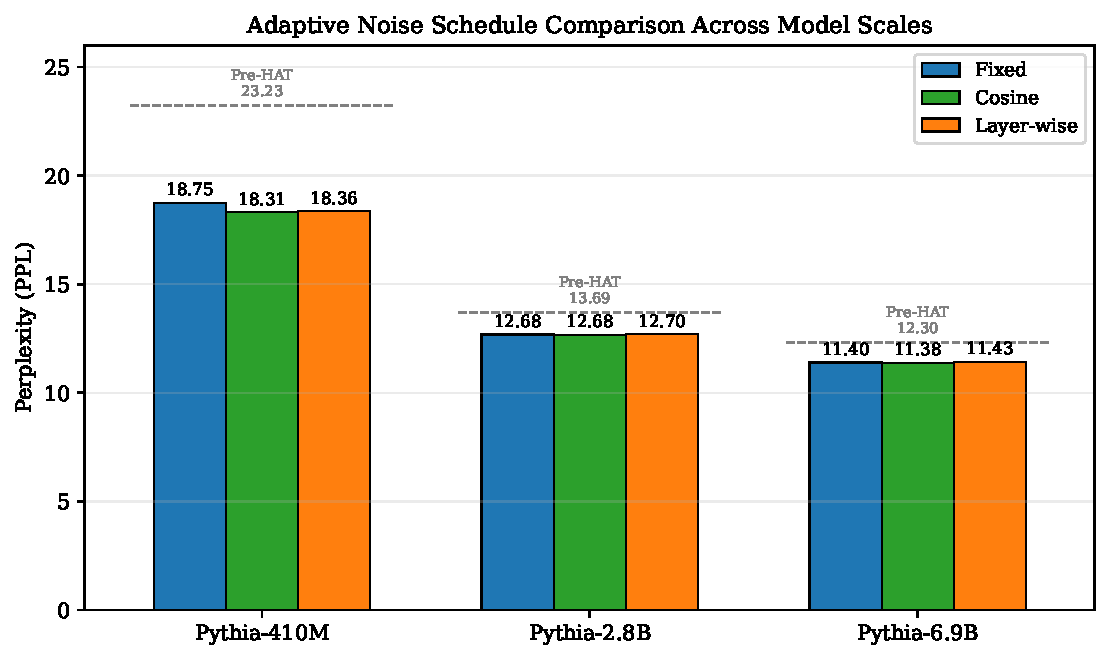
\includegraphics[width=0.90\textwidth]{paper2_fig_remote107_r3_adaptive_ppl_20260513}
\caption{Remote~107 R3 自适应噪声调度比较。对于冻结非目标参数的 410M 主线，cosine decay 达到最低 PPL=18.31，略优于 layer-wise 的 18.36 和 fixed 的 18.75；reverse layer-wise 退化到 21.30，作为负面对照。对 2.8B 和 6.9B，fixed、cosine 和 layer-wise 之间只保留小幅差异。}
\label{fig:paper2-107-r3-adaptive}
\end{figure}

真正出现结构性收益的是扩大模拟覆盖范围时的调度选择。Pythia-2.8B 的联合消融表明，last1 fixed 为 12.68，last1 cosine 同样为 12.68，last2 fixed 升至 13.78，而 last2+cosine 进一步降到 12.56，成为当前 p28b 路线中的最佳结果；last4 fixed 则回升到 14.12。也就是说，R3 没有推翻“last1 是默认主路线”的结论，而是补充了一条更细的设计规则：若希望把模拟 KV 的覆盖范围从单一终端层扩展到 last2，以换取更高的面积或能效收益，应优先采用自适应 schedule，而不是简单沿用 fixed 训练。

\begin{figure}[!htbp]
\centering
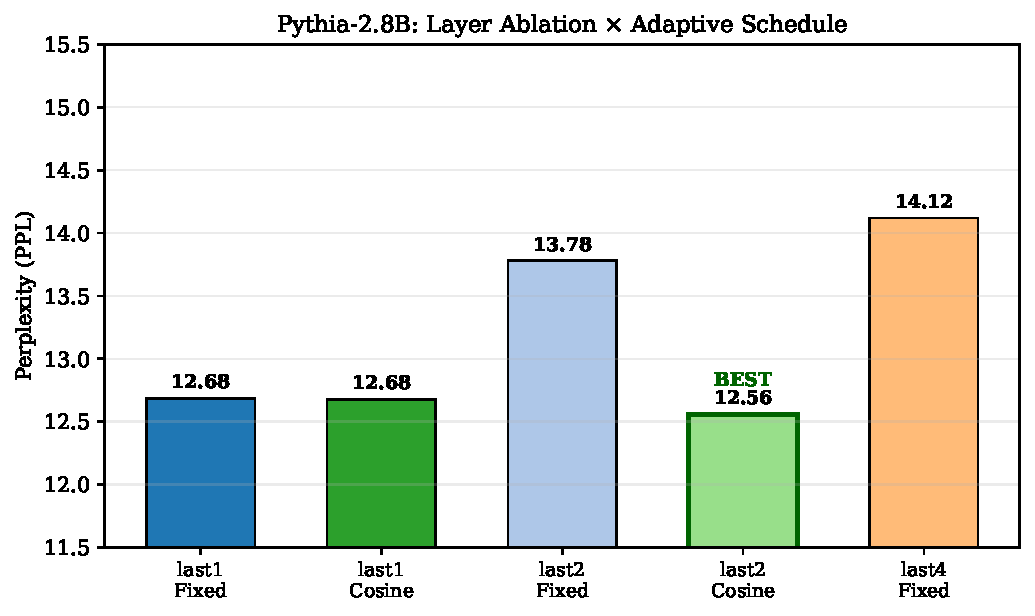
\includegraphics[width=0.82\textwidth]{paper2_fig_remote107_r3_p28b_ablation_20260513}
\caption{Pythia-2.8B 层范围与调度联合消融。last2+cosine 达到最佳 PPL=12.56，优于 last2+fixed 的 13.78，也略优于 last1+fixed 的 12.68。该结果支持把自适应调度作为扩大模拟覆盖范围时的工程补偿手段。}
\label{fig:paper2-107-r3-p28b}
\end{figure}

作为与困惑度不同的离线诊断，图~\ref{fig:paper2-kv-offline-bitwidth} 直接读取 Pythia-410M 的真实 KV 张量，经过量化、固定 D2D 和重复 C2C 读出后计算相对重构均方误差。该结果显示 4-bit 到 6/8-bit 存在明显误差下降，16-bit 接近当前噪声底；last2 与 last4 的 8-bit 相对重构误差约为 $1.2\times10^{-4}$，与 last1 处于同一数量级。这一图只说明张量存储--读出链路的数值误差结构，不能替代端到端 PPL 评估。

\begin{figure}[!htbp]
\centering
\includegraphics[width=0.90\textwidth]{paper2_fig_w2_kv_offline_bitwidth_scan_20260511}
\caption{真实 KV 张量离线重构的位宽诊断。A 显示 last1/last2/last4/all24 在 4、6、8、16-bit 下的相对 KV 重构均方误差，B 比较 8-bit 与 16-bit 的层范围差异。该实验使用真实 Pythia-410M KV 张量和模拟读出噪声，但没有接入注意力前向传播，因此只作为数值诊断而非困惑度证据。}
\label{fig:paper2-kv-offline-bitwidth}
\end{figure}

图~\ref{fig:paper2-kv-retention-refresh} 进一步把离线诊断扩展到时间保持与刷新。该实验使用同一批真实 Pythia-410M KV 张量，在 8-bit、$\sigma_{\mathrm{D2D}}=0.005$、$\sigma_{\mathrm{C2C}}=0.002$ 下扫描会话跨度、保持时间常数和刷新间隔。无刷新且会话跨度远大于 $\tau$ 时，相对重构误差可接近 1，说明缓存态已经显著衰减；当 $\tau=1000$~s 且每 10~s 刷新时，last1/last2/last4/all24 在 1000~s 跨度下的误差回落到约 $10^{-4}$--$10^{-3}$。该图为假设~\ref{hyp:retention} 的数值压力测试提供了方向，但仍没有接入端到端注意力前向传播，也没有核算刷新能耗和耐久预算。

\begin{figure}[!htbp]
\centering
\includegraphics[width=0.90\textwidth]{paper2_fig_w2_kv_retention_refresh_scan_20260511}
\caption{真实 KV 张量离线重构的保持--刷新诊断。A 显示 1000~s 会话跨度且无刷新时，相对 KV 重构误差随保持时间常数 $\tau$ 改善；B 显示在 $\tau=1000$~s 下，不同刷新间隔对 1000~s 会话跨度的误差恢复作用。该实验只评估存储--读出链路的时间动态，不构成端到端困惑度或能耗结论。}
\label{fig:paper2-kv-retention-refresh}
\end{figure}

表~\ref{tab:work2_alllayer_sweep} 的 6-bit 全层扫描给出了更强的压力证据：C2C 和 D2D 任一轴增大都会快速推高困惑度，尤其 D2D=0.10 时已完全失去实用意义。500 步 HAT 预热可把全层 PPL 从 579.52 降至 142.27，但仍远未通过门限，因此 HAT 资源应集中在选择性终端层，而非全层救援。

\begin{table}[!htbp]
\centering
\caption{6-bit 全层噪声敏感性扫描（seed=42）。}
\label{tab:work2_alllayer_sweep}
\begin{tabular}{@{}lcccccc@{}}
\toprule
$\sigma_{\text{c2c}}$ & 0.0 & 0.005 & 0.01 & 0.015 & 0.02 & 0.03 \\
PPL & 32.41 & 39.86 & 56.73 & 77.36 & 100.64 & 160.34 \\
\midrule
$\sigma_{\text{d2d}}$ & 0.0 & 0.01 & 0.02 & 0.05 & 0.10 & \\
PPL & 32.41 & 60.30 & 106.48 & 470.92 & 7635.49 & \\
\bottomrule
\end{tabular}
\end{table}

Fresh-D2D 交叉实例验证进一步支持选择性路线。训练时固定 D2D=0.02，评估时在 5 个独立 D2D 种子上重复。表~\ref{tab:work2_fresh_d2d} 显示，last1 在 eval D2D=0.02--0.05 范围内仅从 18.42 增至 18.60，标准差始终低于 0.03；last2 从 18.71 增至 19.21，仍表现出低方差但均值略高；全层则从 26.05 增至 66.84，且跨实例方差快速扩大。当前路线排序因此是 last1 为主、last2 为备选、全层仅作压力测试。高 D2D 训练对全层有一定收益，例如 D2D=0.04 训练在 eval 0.05 时优于 D2D=0.02 训练，但对 last1 没有明显必要。

\begin{table}[!htbp]
\centering
\caption{选择性终端层 Fresh-D2D 交叉实例验证（train D2D=0.02, seed=42）。}
\label{tab:work2_fresh_d2d}
\begin{tabular}{@{}lcccccc@{}}
\toprule
配置 & 评估 D2D & $n$ 种子 & 均值 PPL & 标准差 & min & max \\
\midrule
last1 [23] & 0.02 & 5 & 18.42 & 0.02 & 18.40 & 18.45 \\
last1 [23] & 0.04 & 5 & 18.55 & 0.03 & 18.52 & 18.58 \\
last1 [23] & 0.05 & 5 & 18.60 & 0.03 & 18.56 & 18.63 \\
\midrule
last2 [22,23] & 0.02 & 5 & 18.71 & 0.02 & 18.69 & 18.74 \\
last2 [22,23] & 0.04 & 5 & 19.07 & 0.04 & 19.03 & 19.13 \\
last2 [22,23] & 0.05 & 5 & 19.21 & 0.04 & 19.17 & 19.26 \\
\midrule
全层 & 0.02 & 5 & 26.05 & 0.53 & 25.17 & 26.50 \\
全层 & 0.04 & 5 & 44.34 & 2.65 & 40.08 & 46.74 \\
全层 & 0.05 & 5 & 66.84 & 5.91 & 57.65 & 73.06 \\
\bottomrule
\end{tabular}
\end{table}

这些结果阶段性支持假设~\ref{hyp:precision} 在选择性终端层范围内成立：当 $\sigma_{\text{d2d}}\le0.05$ 且量化为 8-bit 时，last1/last2 的困惑度退化处于可继续优化的范围，并且 fresh-D2D 方差很低。假设~\ref{hyp:retention} 和假设~\ref{hyp:endurance} 尚需时间动态和刷新实验确认，因此器件物理匹配目前应被表述为有先验支撑的候选优势，而不是最终部署结论。

\FloatBarrier

\section{贡献、边界与后续判据}
\label{sec:work2_contributions}
\label{sec:work2_boundaries}

Work~2 与 Work~1 的关系不是重复证明有机 CIM 可以运行神经网络，而是寻找更适合其物理特性的负载。Work~1 说明，动态激活路径、全局注意力和固定 D2D 实例会把有机阵列的非理想性放大为部署风险；Work~2 则转向静态 KV 缓存，利用其低频写入、高频读取和会话级生命周期。若选择性终端层路线在后续复现中继续成立，本文的知识增量在于说明同一种器件物理在不同负载下可从限制因素转化为候选优势。方法论增量在于把器件保持时间、耐久性、噪声和刷新机制映射到 LLM 困惑度、任务指标和能效，而不是只报告单器件指标或孤立的矩阵乘法误差。

当前边界见表~\ref{tab:boundaries}。这些排除项并不否定未来可扩展性，而是防止把行为级仿真和 1--3B 模型上的结论外推到尚未验证的系统规模。尤其是 $>$7B 模型、多片芯粒互连、128k 上下文和光电前端联合训练都可能成为后续工作，但它们需要新的容量模型、调度策略和硬件假设，不能由本章数据直接支撑。

\begin{table}[!htbp]
\centering
\caption{范围边界与排除理由。}
\label{tab:boundaries}
\small
\begin{tabularx}{\textwidth}{@{}l>{\raggedright\arraybackslash}X@{}}
\toprule
排除项 & 理由 \\
\midrule
$>$7B 参数模型 & 当前有机交叉阵列密度和仿真成本不足以支撑完整 KV 缓存评估；多片划分属于系统架构问题 \\
$>$32k token 上下文 & 超长上下文需要 3D 堆叠、混合存储层级或片外卸载，不再只考察有机 CIM 本征物理 \\
KV 缓存片上训练 & 训练需要高频原地更新 K/V 张量，超出 $10^3$--$10^4$ 次耐久假设 \\
生产部署声明 & 本章是行为级仿真和路线筛选，不给出商用部署承诺 \\
完整光电协同设计 & 光子前端与 CIM 权重联合训练属于更宽的前端方向，不作为本章独立贡献 \\
多片/芯粒扩展 & 芯粒互连和跨片调度属于工程外延，仅在架构探索中作为约束讨论 \\
\bottomrule
\end{tabularx}
\end{table}

后续判断标准也应保持可审计。当前选择性 KV 锁定包已完整归档 last1 至 all24 的逐行命令、检查点哈希、seed 语义和 JSON 文件，因此可用于支持层范围排序和全层负面对照结论；但时间动态实验仍需给出 $\tau$、刷新间隔、能耗和困惑度之间的曲线，才能继续支撑假设~\ref{hyp:retention} 和假设~\ref{hyp:endurance}。若这些实验不支持长期会话，本章结论应收缩为短会话或低层覆盖范围内的原型级可行性。

\FloatBarrier

\section{本章小结}
\label{sec:work2_summary}

本章把有机光电 CIM 从视觉权重映射扩展到 LLM KV 缓存场景。核心逻辑是：KV 缓存具有低频写入、高频读取和会话级生命周期，有机 OEC-RAM 的 $\sim10^3$~s 保持时间、有限耐久性和光学刷新机制与这一负载在数量级上更匹配。Remote~107 早期数据排除了全层模拟 KV 缓存作为主路线：8-bit 全层零噪声已达 PPL=17.48，相对旧数字基线 15.68 退化 11.5\%；6-bit 全层在 D2D/C2C 扫描中迅速失控。当前 selective-KV claim-lock packet 进一步锁定了相同排序：在 Pythia-410M、WikiText-2 raw-v1 test、context 512、non-overlapping stride 512、batch size 1 下，数字基线为 PPL=23.30；last1/last2 在 D2D=0.02--0.05 下保持在约 18.6--19.0 PPL，last4 升至约 20.4--21.5 PPL，而 all24 在 D2D=0.05 时恶化到 $59.055\pm1.610$ PPL。上述证据支持选择性终端层作为 Work~2 的主候选，并将全层模拟 KV 缓存定位为负面对照；第~\ref{chap:deployment-envelope}~章将回到视觉主线的部署包络，并把 Work~2 当前结论作为有机 CIM 适用性边界的一部分。

% 第7章 部署包络
\chapter{部署包络}
\label{chap:deployment-envelope}

本章将前六章的仿真数据转化为可操作的部署知识，为有机光电存算一体（CIM）阵列上的视觉Transformer落地提供定量边界。
前序章节已建立了HAT分类学、失效模式图谱与缓解策略的完整物理图景；
本章的任务是回答一个工程问题：
在给定的器件参数组合下，Ensemble HAT训练协议能否在未见硬件实例上保持可用的精度排序？
若不能，崩溃边界在哪里？

全章仅使用已冻结的实验数据，所有外推均明确标注不确定度。

\section{部署场景定义}
\label{sec:deployment-scenario}

\subsection{目标应用：边缘视觉推理}

本章的部署包络面向\emph{边缘视觉推理}场景：
在功耗受限的端侧设备上，对 $32\times32$ 至 $224\times224$ 分辨率的图像执行单标签分类。
基准模型为 Tiny-ViT-5M（CIFAR-10 数字基线 $98.06\%$），
阵列映射方式采用第~\ref{chap:methodology}~章所述的混合模拟--数字分区：
注意力 QKV、投影层与 MLP 的权重矩阵部署于有机光电阻变阵列，
层归一化、Softmax 与分类头保留数字实现。

\subsection{CIM 阵列规模与外围约束}

仿真框架将每个模拟层视为独立的交叉阵列瓦片（crossbar tile）。
以 Tiny-ViT-5M 为例，全模型共 $42$ 个可映射的模拟层，
其中 Attention QKV $10$ 层、Attention Projection $10$ 层、FFN (fc1+fc2) $20$ 层、Patch Embedding $2$ 层。
层敏感度扫描（冻结数据，见 \texttt{layer\_sensitivity\_results\_gpt.json}）表明，
在标准 HAT 检查点上对各层组单独注入 $5\%$ C2C 噪声时，
各组孤立精度均维持在 $91.61\%$--$91.72\%$ 区间，
差异小于 $0.11$~pp，说明在 canonical 均匀噪声下没有单一\emph{层组}构成明显的精度瓶颈。

进一步的全 $42$ 层单层 D2D 重采样 pilot 扫描显示，逐层风险并非均匀分布。
该扫描冻结 V4 检查点与其余层的 D2D 缓冲，仅对一个目标模拟层重新采样 $\sigma_{\mathrm{D2D}}=10\%$ 失配，
并在 $512$ 张 CIFAR-10 子集、$3$ 个随机种子上估计精度掉点（见
\texttt{layer\_sensitivity\_full42\_summary\_20260510.tsv}）。
结果呈现明显 heavy-tail：末级 MLP 输出层 \texttt{stages.3.blocks.0.mlp.fc2} 的平均掉点达到 $83.59$~pp，
而第二敏感层为 $26.24$~pp，多数 attention projection 与后段 attention 层低于 $1$~pp。
该证据仍为 \texttt{pilot/provisional}，不能替代完整测试集或 fresh-instance 协议；
但它提示混合精度或冗余保护不应平均分配到所有阵列，而应优先覆盖少数 catastrophic outlier。

\begin{figure}[t]
    \centering
    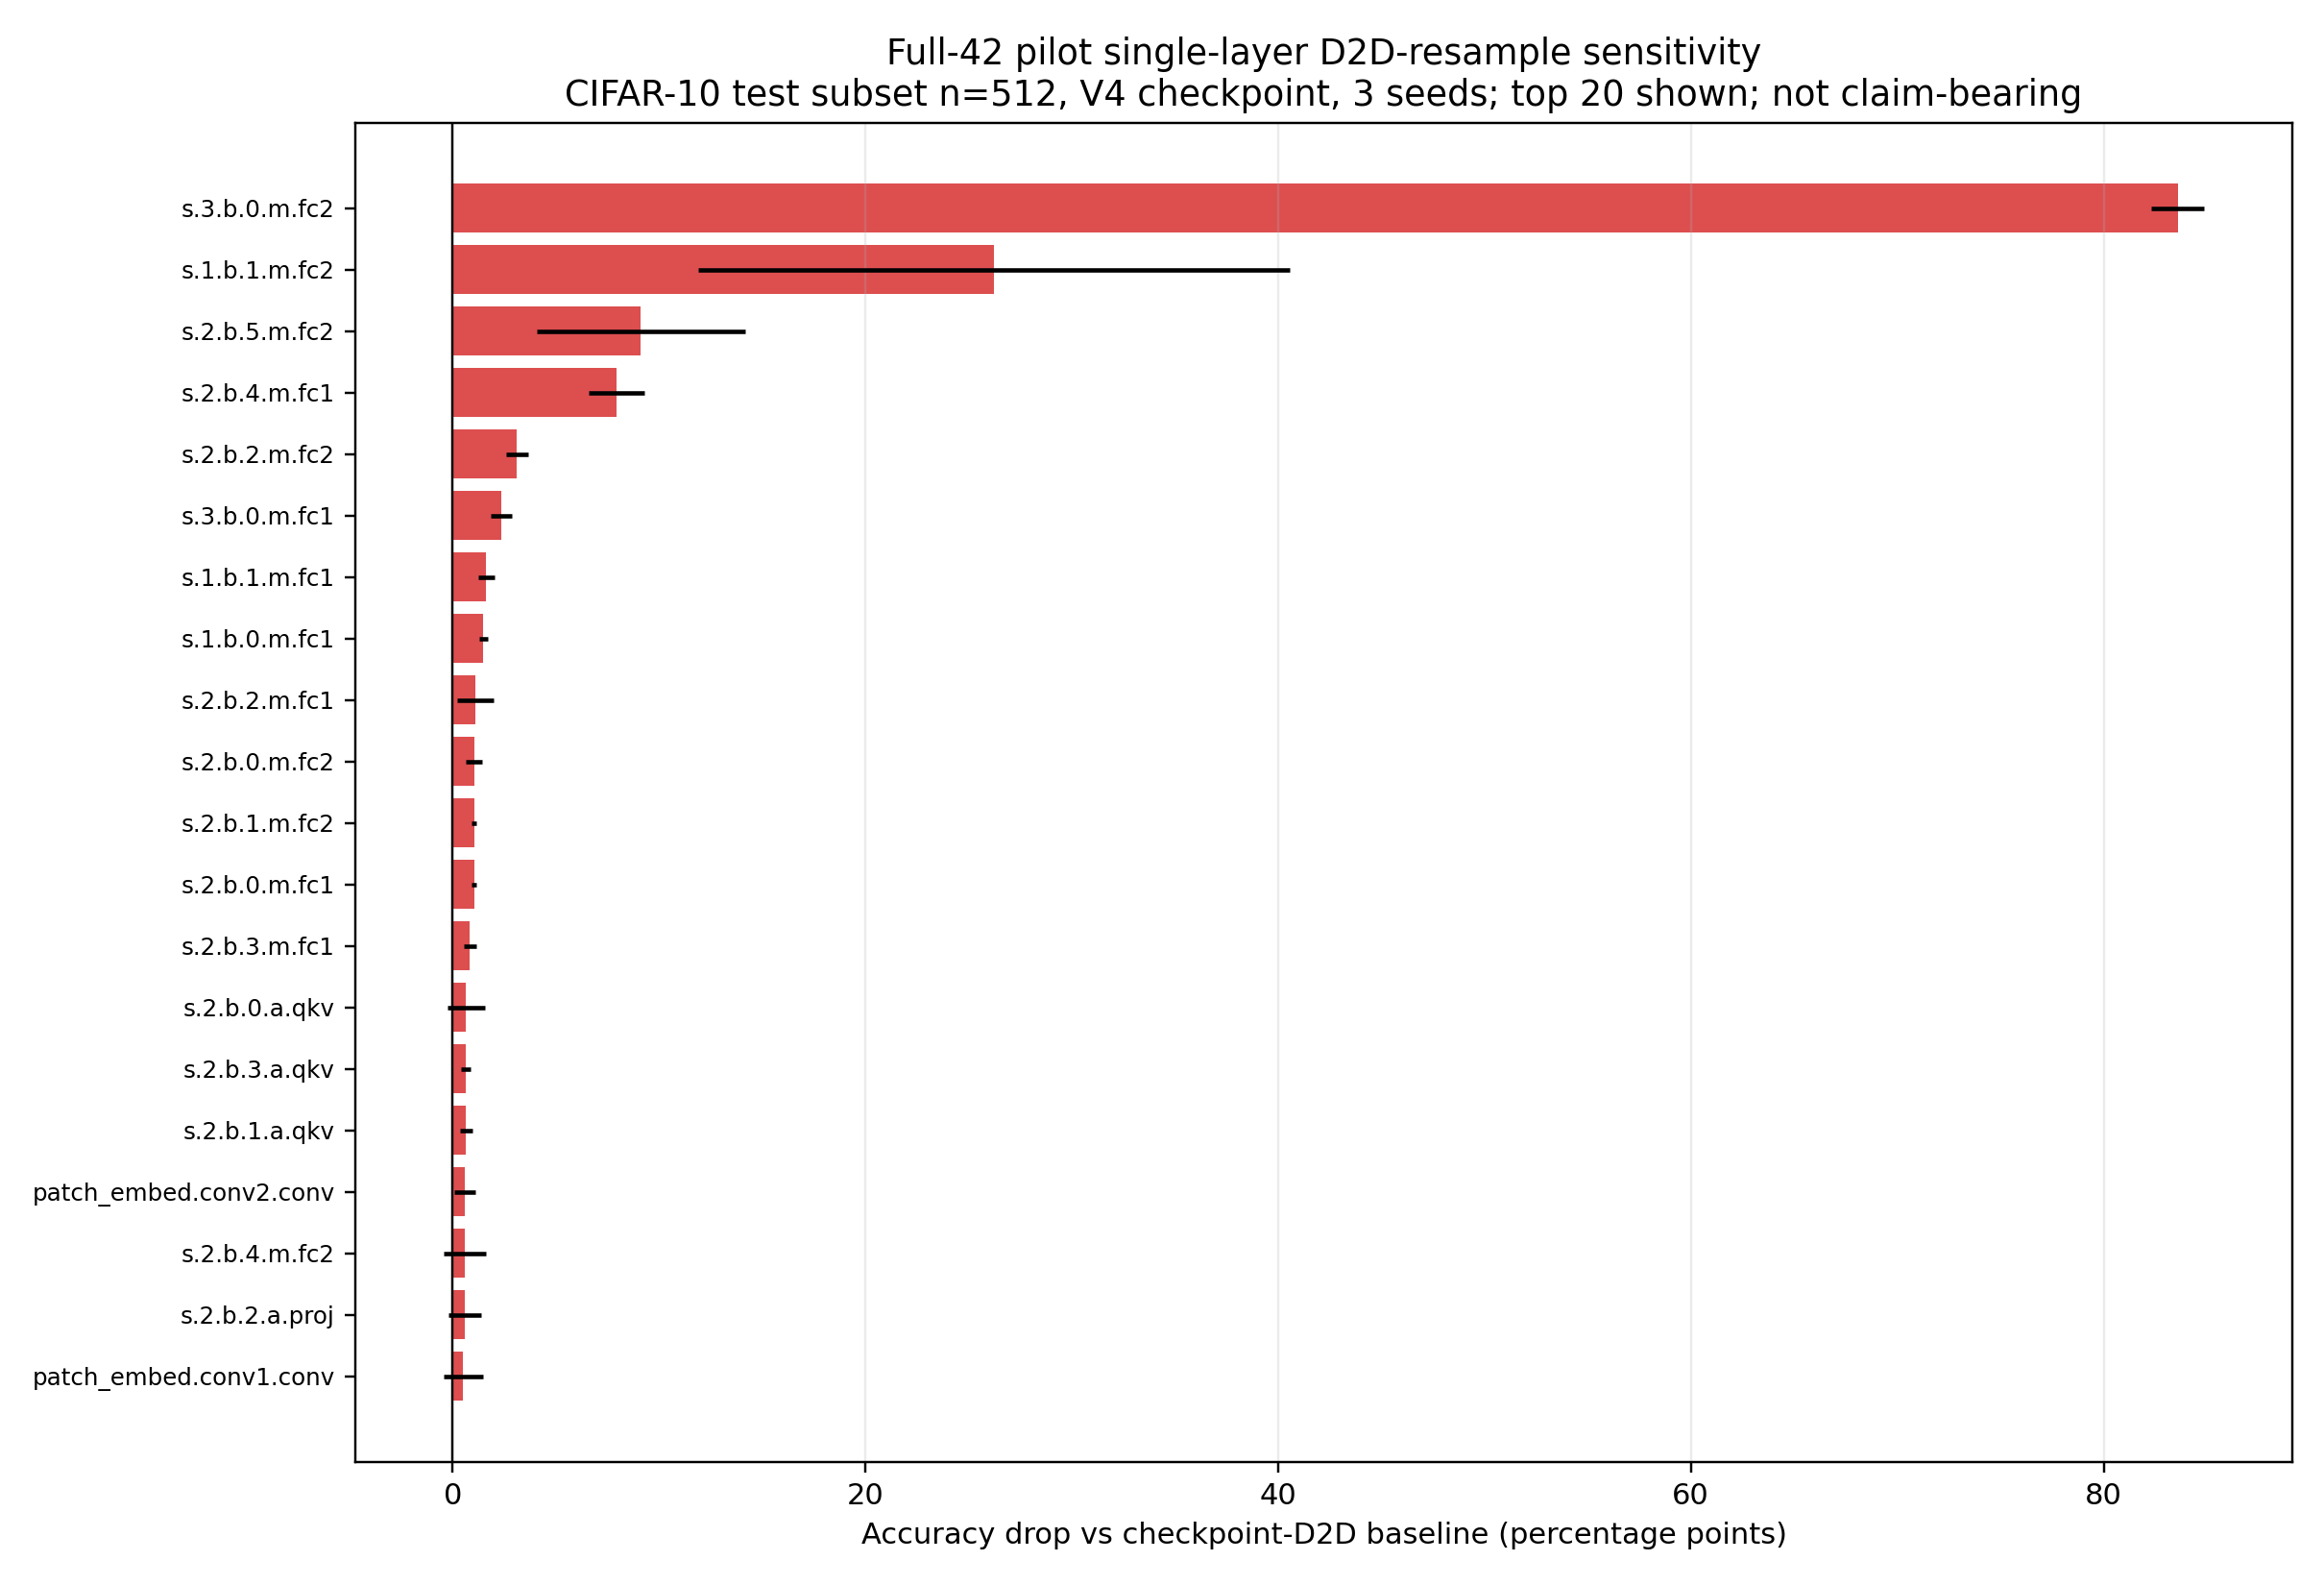
\includegraphics[width=0.95\textwidth]{fig_layer_sensitivity_full42_20260510}
    \caption{全 $42$ 个可映射模拟层的单层 D2D 重采样敏感度 pilot。每次仅重采样一个目标层，其余层恢复到 V4 检查点 D2D 缓冲；精度掉点在 $512$ 张 CIFAR-10 子集与 $3$ 个种子上统计。该图用于定位混合精度保护候选，不作为最终 claim-bearing 验证。}
    \label{fig:full42-layer-sensitivity}
\end{figure}

为检验该排序是否能转化为部署保护策略，本研究追加了一个 full-test provisional 保护曲线：
在完整 $10{,}000$ 张 CIFAR-10 测试集与 $3$ 个种子上，将所有模拟层重采样为 fresh D2D 实例，
然后把 full42 排名前 $K$ 的敏感层保留在 checkpoint D2D（\texttt{freeze\_topK\_d2d}），其余层仍使用 fresh D2D。
结果如图~\ref{fig:protection-map-fulltest} 所示。
完全 fresh 的全模拟模型为 $10.00\%$，对应随机猜测；保护前 $10$ 层提高到 $22.44\pm3.74\%$，
前 $13$ 层提高到 $34.81\pm3.09\%$，前 $20$ 层提高到 $65.93\pm2.88\%$，
前 $30$ 层达到 $86.06\pm0.23\%$，距离全 checkpoint D2D 的 $91.96\pm0.20\%$ 仅约 $5.90$~pp。
这说明 full42 排序确实携带强定位信号：风险集中在一个长尾子集内，而非平均分布于全部 $42$ 个阵列层。
但该协议仍是推理期 D2D 保留/重采样诊断，不等同于真实工艺中的混合精度实现，也不是多硬件实例 fresh-instance 训练评估。
因此，混合精度策略在本文中应定位为候选部署设计：若外围或工艺预算允许优先保护约 $30/42$ 个高敏感层，
则有望接近源域性能；若只保护前 $10$--$13$ 个 catastrophic outlier，则仍不足以解除固定掩膜模型的部署崩溃。

\begin{figure}[t]
    \centering
    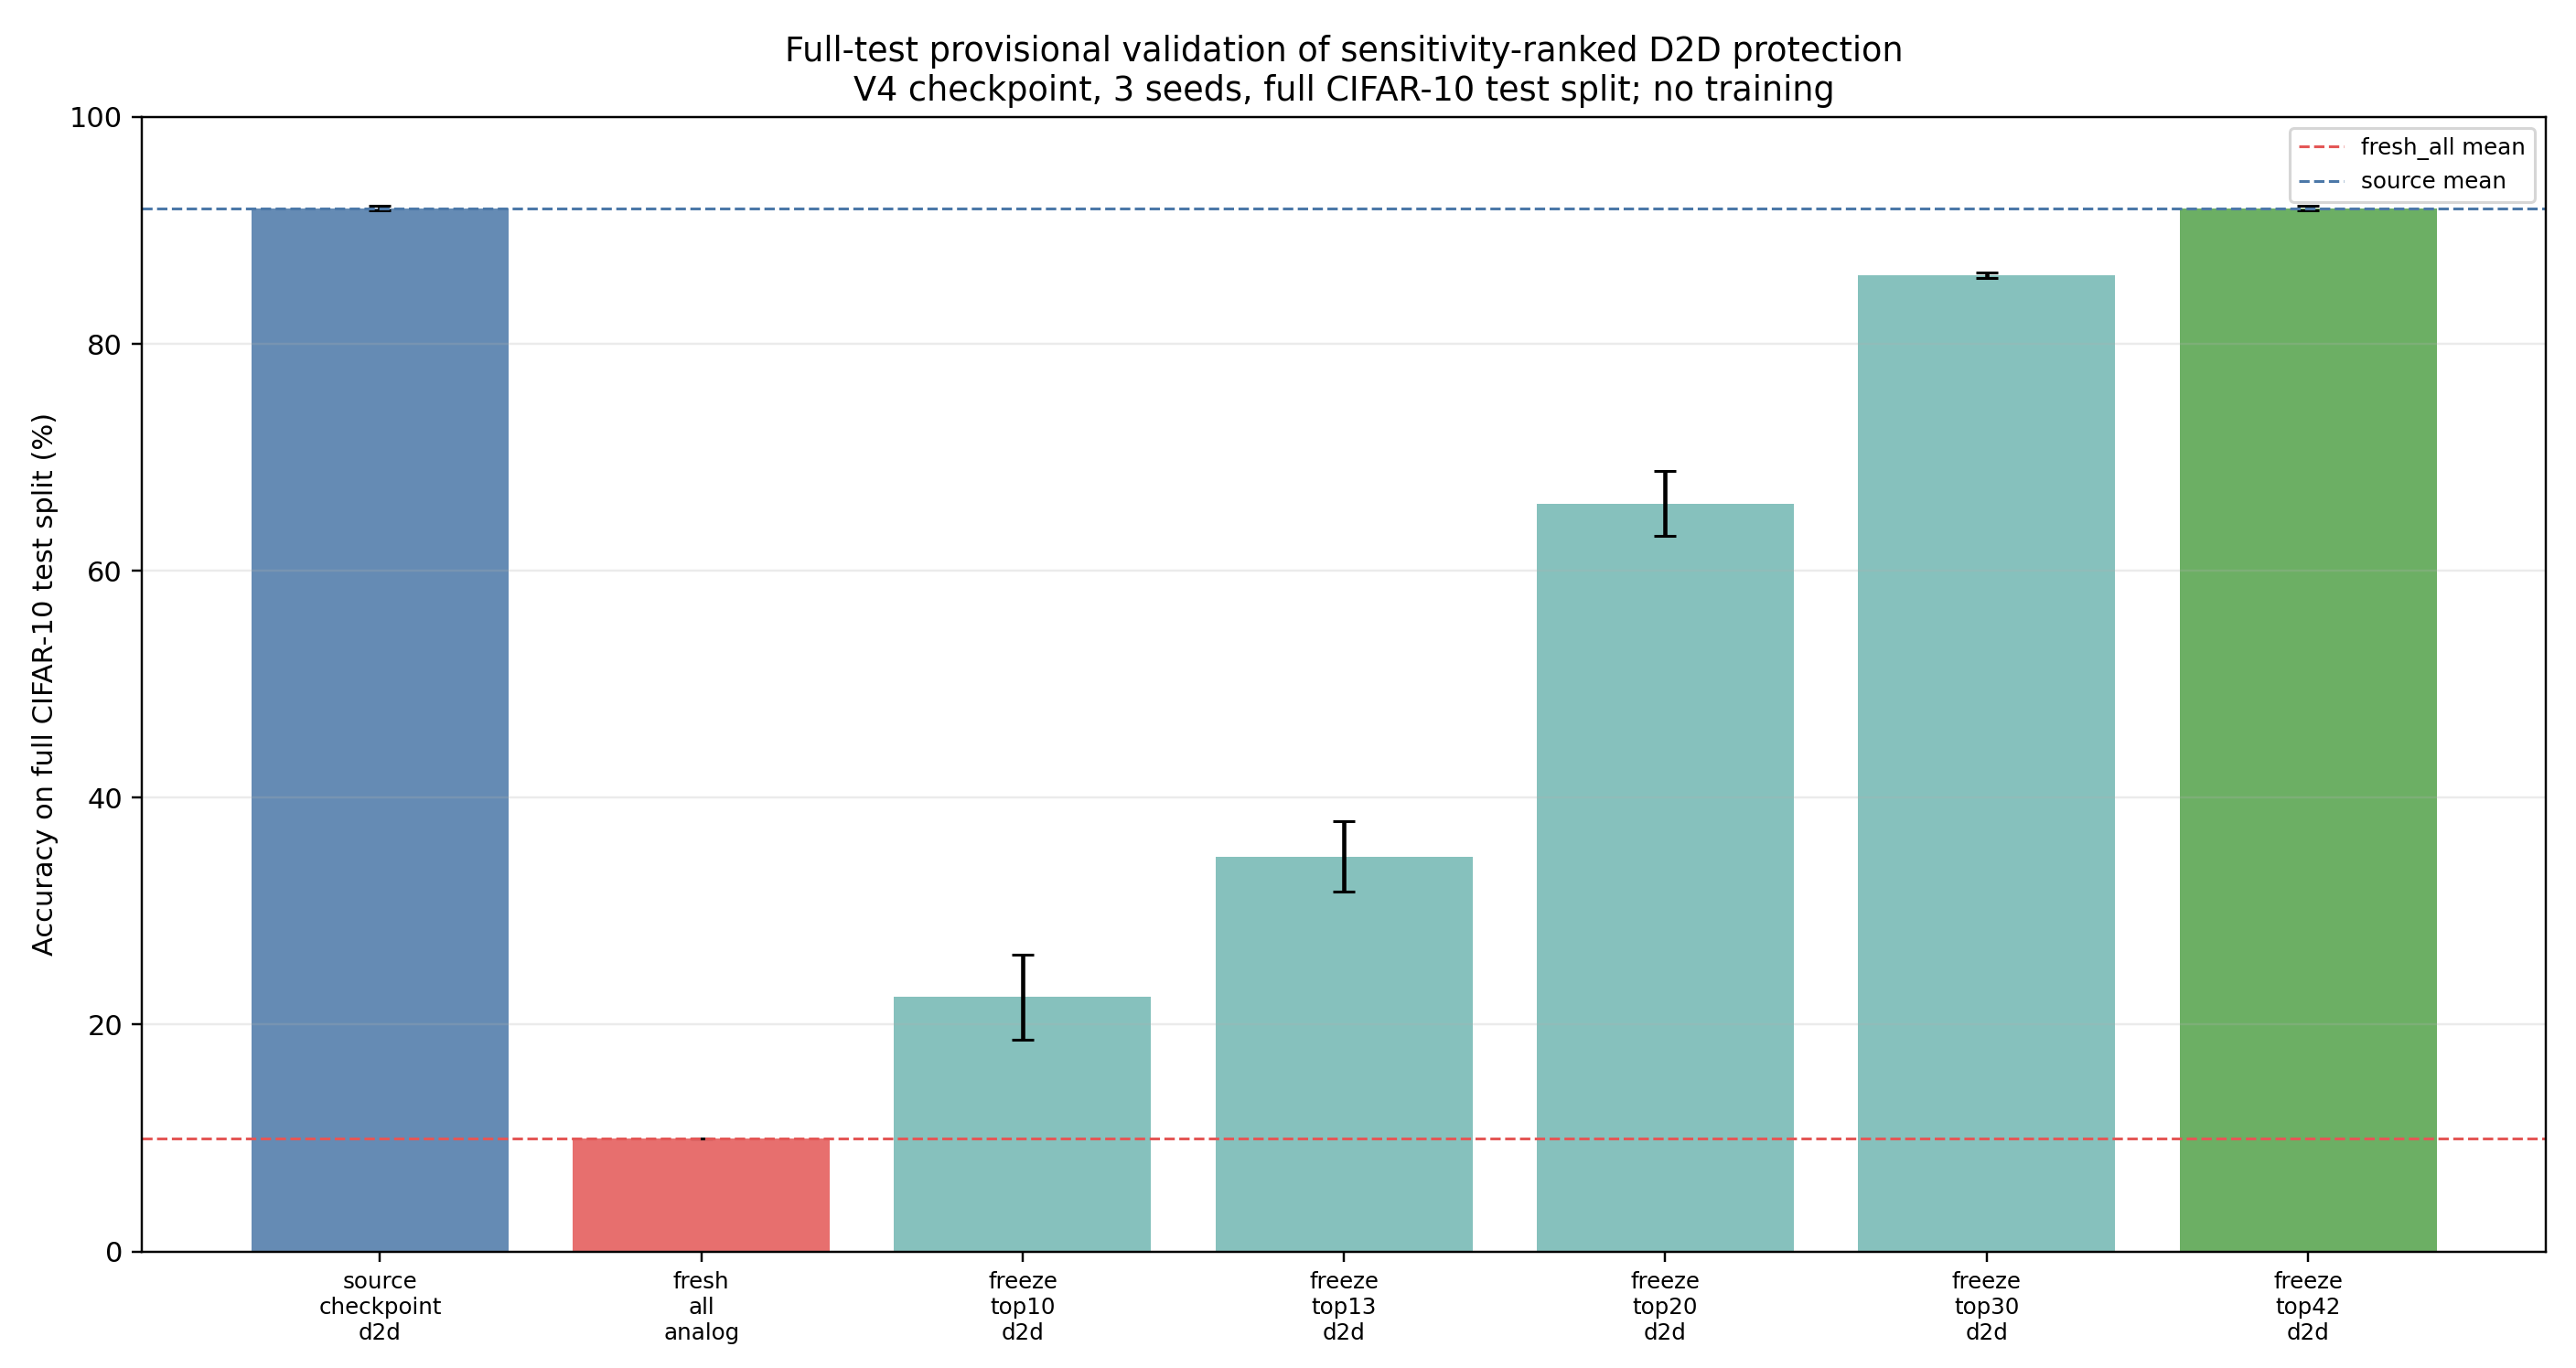
\includegraphics[width=0.95\textwidth]{fig_protection_map_fulltest_p1_20260510}
    \caption{基于 full42 排序的完整 CIFAR-10 测试集保护曲线。\texttt{freeze\_topK\_d2d} 将排名前 $K$ 的敏感层保留为 checkpoint D2D，其余层重采样为 fresh D2D。结果显示 top-$30$ 保护可恢复到 $86.06\pm0.23\%$，但该图仍为推理期定位诊断，不是最终 fresh-instance 部署验证。}
    \label{fig:protection-map-fulltest}
\end{figure}

外围读出电路的能效约束通过一阶解析模型估算。
在 $8$~bit ADC、$100$ 个阵列、$1000$ 次转换的基准假设下，
系统总能量约为 $23.9$~$\mu$J（FP32 数字基线约 $273.94$~$\mu$J），
对应相对 FP32 的加速比约为 $11.45\times$，
相对假设 INT8 的加速比约为 $2.86\times$
（见 \texttt{energy\_scale\_recovery\_sensitivity.json}）。
该估算为一阶解析假设，非流片测量值；
实际部署需根据具体 CMOS 工艺节点重新标定。

\subsection{功耗约束与刷新策略}

有机阵列的保留漂移（retention drift）引入时间维度上的功耗--精度权衡。
V8 保留轨迹显示：$t=0$~s 时源域精度为 $91.63\%$，
$t=1$~s 骤降至 $82.66\%$，随后在 $10$~s 至 $10{,}000$~s 区间形成 $79.13$--$79.51\%$ 的宽平台。
若应用要求 $>82\%$ 精度，则动态标度重校准的刷新间隔须短于约 $1$~s；
若可接受 $79\%$ 精度，则间隔可延长至数小时。
该任务依赖性刷新规格直接影响外围参考单元读出电路的能耗预算。


\section{ADC 分辨率包络}
\label{sec:adc-envelope}

\subsection{6-bit 悬崖：量化主导区与 D2D 主导区的分界}

ADC 精度是决定系统能否脱离近随机猜测状态的首要参数。
在 $63$ 点联合扫描（$\sigma_{\mathrm{D2D}} \in \{1,3,5,8,10,15,20\}\%$，
ADC $\in \{2,3,4,5,6,7,8,10,12\}$~bit，C2C=$5\%$，$NL=1.0$，
每点 $10$ 次蒙特卡洛运行）中，
精度随 ADC 位宽呈现明显的两阶段结构（见 \texttt{iso\_accuracy\_contour\_data.json}）：

\begin{itemize}
    \item \textbf{亚 5-bit 区}：所有 D2D 水平下精度均接近随机（$\sim$$10\%$--$15\%$）。
    3-bit ADC 在 $10\%$ D2D 下均值仅 $13.62\%$；
    2-bit ADC 在所有 D2D 水平下均低于 $12\%$。
    \item \textbf{5--6-bit 过渡区}：存在约 $7$~pp 的陡峭跳变。
    以 $10\%$ D2D 为例，5-bit 均值 $76.85\%$，6-bit 跃升至 $84.77\%$，
    增量达 $7.92$~pp；
    七个 D2D 级别的平均跳变为 $\sim$$7$~pp（单行间 $5.8$--$8.1$~pp）。
    \item \textbf{$\ge$6-bit 操作区}：精度退化由 D2D 主导。
    在 $10\%$ D2D 下，6-bit 为 $84.77\%$，8-bit 为 $87.12\%$，
    12-bit 为 $86.98\%$；继续提升 ADC 位宽收益递减。
\end{itemize}

\subsection{Sobol 全局敏感度分解}

为定量区分 ADC 精度与 D2D 失配的相对贡献，
对联合扫描数据执行一阶 Sobol 敏感度分析
（见 \texttt{sobol\_sensitivity.json}）：

\begin{itemize}
    \item \textbf{全参数网格}（含亚 5-bit 区）：
    $S_{\mathrm{ADC}} = 0.976$，$S_{\mathrm{D2D}} = 0.018$，
    交互项 $S_{\mathrm{inter}} = 0.006$。
    ADC 位宽解释了约 $97.6\%$ 的精度方差，
    说明在跨越悬崖的宏观尺度上，读出精度是压倒性主因。
    \item \textbf{操作区}（ADC $\ge$ 6-bit 且 $\sigma_{\mathrm{D2D}} \le 15\%$）：
    $S_{\mathrm{ADC}} = 0.041$，$S_{\mathrm{D2D}} = 0.922$，
    交互项 $S_{\mathrm{inter}} = 0.038$。
    一旦越过 6-bit 悬崖，D2D 失配立即成为剩余方差的 $92.2\%$ 来源。
\end{itemize}

该两阶段结构具有明确的工程含义：
\textbf{6-bit ADC 是当前混合架构的最小可行外围}。
低于 5-bit，无论训练协议如何精进，系统均无法脱离随机水平；
高于 6-bit，投资回报比的排序变为 D2D 均匀性 $>$ ADC 位宽。

\subsection{ADC 非理想性的边际效应}

在 8-bit 基线上，对偏移、增益误差与积分非线性（INL）的独立扫描
（见 \texttt{adc\_nonideality\_final.json}）显示：
$\pm 0.5$~LSB 偏移几乎无影响（$63.02\%$ vs 理想 $63.04\%$）；
$\pm 5\%$ 增益误差导致 $-0.77$~pp；
$0.5$~LSB INL 无影响；
组合现实场景（$\pm 0.5$~LSB 偏移 $+5\%$ 增益误差 $+0.5$~LSB INL）
仅下降 $-0.75$~pp 至 $62.29\%$。
这些非理想性在绝对数值上远小于 6-bit 悬崖的 $7$~pp 跳变，
说明在部署包络中，\emph{位宽本身比位宽内的线性度更重要}。


\section{D2D 失配包络}
\label{sec:d2d-envelope}

\subsection{固定掩膜 HAT 的硬件实例过拟合}

标准 HAT（固定掩膜，fixed-mask）在训练时阵列上可达 $87.95\pm0.27\%$，
但在 $10$ 个全新硬件实例上的 fresh-instance 评估中，
精度 deterministic 地崩塌至 $10.00\pm0.00\%$。
该结果已在 AMP 关闭的 FP32 推理路径上独立复现，
确认其为优化器耦合到特定空间失配图 $M_0$ 的结构性后果，
而非数值 artifact。

该崩塌是\textbf{绝对的}：
它不因 D2D 幅度降低而改善。
在文献标定的 OPECT 低噪声代理（$\sigma_{\mathrm{D2D}}=3\%$，$\sigma_{\mathrm{C2C}}=2\%$）下，
标准 HAT 检查点同样崩塌至 $10.00\%$。
因此，对于任何要求跨实例鲁棒性的有机 RRAM 工艺，
\textbf{固定掩膜 HAT 不可作为部署候选}。

\subsection{Ensemble HAT 的跨实例统计}

Ensemble HAT 通过每轮epoch重采样 D2D 失配图，
将实例分布烘焙进训练目标。
在相同的 $10$ 实例 $\times$ $5$ MC 评估协议下，其结果为：

\begin{itemize}
    \item \textbf{Canonical 均匀噪声}（$\sigma_{\mathrm{D2D}}=10\%$，i.i.d.）：
    $86.16\pm0.19\%$（见 canonical fresh-instance 评估记录）。
    \item \textbf{中度空间相关 D2D}（$\rho=0.3$，可分 AR(1) 模型，zone 3A 免疫协议，NL=1.0，AMP 关闭）：
    $84.57\pm2.39\%$
    （见 \texttt{fresh\_instance\_eval\_v4\_ensemble\_correlated\_d2d.json}）。
    相对 i.i.d.~基线仅下降 $1.76$~pp，排序保持。
    \item \textbf{强空间相关 D2D}（$\rho=0.5$，zone 3A 免疫协议）：
    $82.12\pm3.95\%$
    （同前）。
    相对基线下降 $4.20$~pp，但最差实例仍为 $73.7\%$，远离随机水平。
\end{itemize}

\begin{table}[t]
\centering
\caption{D2D 失配包络：标准 HAT 与 Ensemble HAT 的 fresh-instance 精度对比（CIFAR-10 top-1，$10 \times 5$ 协议）}
\label{tab:d2d-envelope}
\small
\begin{tabular}{@{}lccc@{}}
\toprule
\textbf{D2D 条件} & \textbf{标准 HAT} & \textbf{Ensemble HAT} & \textbf{差值} \\
\midrule
i.i.d.~$10\%$ D2D & $10.00\pm0.00$ & $86.16\pm0.19$ & $+76.16$~pp \\
OPECT 代理 $3\%$ D2D & $10.00\pm0.00$ & $88.53\pm0.08$ & $+78.53$~pp \\
空间相关 $\rho=0.3$ & $10.00$（外推） & $84.57\pm2.39$ & $+74.57$~pp \\
空间相关 $\rho=0.5$ & $10.00$（外推） & $82.12\pm3.95$ & $+72.12$~pp \\
\bottomrule
\end{tabular}
\end{table}

表~\ref{tab:d2d-envelope}~表明，
Ensemble HAT 的精度优势不依赖于 $10\%$ D2D 的特定假设：
在低噪声文献代理和高空间相关性两种极端条件下，
排序均稳定保持，且跨实例标准差随相关性增强而增大
（$0.19$~pp $\to$ $3.95$~pp），均值相应下降。


\section{噪声--非线性权衡}
\label{sec:noise-nl-tradeoff}

\subsection{严重非线性写入的恢复带}

写入非线性（$NL$）是第二道硬边界，但修订梯度缩放配方后，其影响呈\emph{系统性退化}而非\emph{结构性崩塌}。
在 $NL=2.0$、canonical 均匀噪声下，M系列6次训练（Standard/Ensemble$\times$Uniform/Proportional$\times$2种子）的 fresh-instance 结果如下（见 \texttt{nl\_postfix\_recovery\_band.json}）：

\begin{itemize}
    \item \textbf{Standard HAT}（固定掩码，均匀噪声，M1/M5）：
    均值 $\mathbf{81.2\%}$，跨实例标准差 $<2$~pp；
    \item \textbf{Ensemble HAT}（均匀噪声，M2/M6）：
    均值 $\mathbf{80.7\%}$，跨实例标准差 $<2$~pp；
    \item \textbf{Ensemble HAT}（比例噪声，M3/M4）：
    均值 $\mathbf{80.7\%}$，跨实例标准差 $<2$~pp。
\end{itemize}

三组配置收敛至同一 $\sim$$80$--$82\%$ 带，差距 $<1$~pp，表明 $NL=2.0$ 下 severe NL 已成为\emph{绑定约束}，训练协议优化收益饱和。

\textbf{ADC-on 与 ADC-off 对比}：
8-bit ADC 开启仅比理想读出低 $\sim$$0.10$~pp（zone 3C），说明读出量化不是主导因素。

\textbf{6-bit 点检}：
6-bit ADC 点检显示 $-2.8$~pp 悬崖（zone 3C），再次确认 6-bit 为最小可行外围。

\textbf{残余差距}：
相对 $NL=1.0$ 基线（$86.16\%$），$NL=2.0$ 的系统性退化约 $5.7$~pp。
该差距源于状态依赖的 LTP/LTD 不对称缩放重塑了优化景观，使注意力通路的特征几何对 D2D 实现的变化更加敏感。
然而，与先前基于未修订梯度缩放配方报告的 $\sim$$30\%$ 不同，当前修订配方下的 $\sim$$80$--$82\%$ 表明瓶颈是\emph{可量化的代理梯度近似误差}，而非不可逾越的结构壁垒。

\subsection{从 $NL=1.0$ 到 $NL=2.0$ 的系统性退化}

$NL=1.0$ 时 Ensemble HAT fresh-instance 精度为 $86.16\%$，
$NL=2.0$ 时降至约 $80.7\%$（Ensemble HAT，均匀噪声）。
退化幅度约 $5.7$~pp，呈单调趋势。
梯度缩放替代模型在 $NL$ 增大时产生状态依赖的 LTP/LTD 不对称缩放，
该不对称性重塑了优化景观，但并未导致灾难性崩塌。
保守边界为：\textbf{$NL=2.0$ 处于可用但次优区}，$NL \ge 2.5$ 的实验数据尚缺，不建议外推。


\section{跨器件零样本迁移}
\label{sec:cross-device-transfer}

\subsection{文献标定器件：OPECT 代理}

作为文献锚定的参考点，
将 Ensemble HAT 检查点零样本迁移至 Zhang et al.~(2025) 报道的 OPECT 阵列代理
（$\sigma_{\mathrm{D2D}}=3\%$，$\sigma_{\mathrm{C2C}}=2\%$，动态范围 $47.3$，$34$ 电导态）
（见 \texttt{literature\_profile\_eval.json} 与 \texttt{ensemble\_literature\_profile\_eval.json}）：
\begin{itemize}
    \item Ensemble HAT：$\mathbf{88.53\pm0.08\%}$（$n=10$ fresh-instance 评估）。
    \item 标准 HAT：$\mathbf{10.00\pm0.00\%}$，同样 deterministic 崩塌。
\end{itemize}

$88.53\%$ 距数字 FP32 基线（$98.06\%$）仍差约 $9.5$~pp，
但已比标准 HAT 的崩塌高出约 $78.5$~pp。
该结果同时设定了当前 Tiny-ViT 架构在接近理想模拟条件下的\emph{精度天花板}：
约 $88.5\%$，跨实例标准差仅 $0.08$~pp，
小于 CIFAR-10 测试集本身的采样噪声。

\subsection{内部实测器件：Doctor OECT}

对内部实测的非易失 OECT 器件配置文件（源自内部PPT原始数据导出）
执行相同协议（见 \texttt{doctor\_measured\_profile\_eval.json}）：
\begin{itemize}
    \item RC-16 配置（$16$ 态，动态范围 $5.75$）：
    Ensemble HAT $89.8\%$；标准 HAT $10.2\%$。
    \item RC-64 配置（$64$ 态，动态范围 $6.18$）：
    Ensemble HAT $89.2\%$；标准 HAT $10.2\%$。
\end{itemize}

实测器件的 D2D 几乎为零（$\sigma_{\mathrm{D2D}}=0$），C2C 亦低于 $0.37\%$，
因此精度高于 OPECT 文献代理，
但标准 HAT 仍崩塌至 $10.2\%$，
再次确认\textbf{硬件实例过拟合风险不随器件均匀性改善而自动消失}。

\subsection{跨仿真器验证：CrossSim 基准}

为验证框架结果的外部一致性，
在 ConvNeXt-Tiny C4 检查点上与 CrossSim~\parencite{crosssim2026} 执行同参数对比
（见 \texttt{crosssim\_standard\_noise.json}，
$\sigma_{\mathrm{C2C}}=5\%$，$\sigma_{\mathrm{D2D}}=5\%$，8-bit ADC，4-bit 权重，$n=3$ 种子）：
\begin{itemize}
    \item 本框架（含 fresh D2D 重采样 + ADCQuantHookManager）：
    $\mathbf{81.63\pm0.56\%}$。
    \item CrossSim（通用编程误差/读取噪声映射）：
    $67.20\pm2.67\%$。
\end{itemize}

在零噪声基线（\texttt{crosssim\_clean\_baseline.json}）下，
本框架 $86.2\%$，CrossSim $83.7\%$，差距缩小至 $2.5$~pp；
在低噪声（$1\%$ D2D/C2C）下，本框架 $85.9\%$，CrossSim $82.9\%$。
差距主要来源于噪声映射方式：
本框架采用固定 D2D + 每前向 C2C 的显式分离，
而 CrossSim 使用统一编程误差/读取噪声幅度，
在高噪声区对失配结构的建模更保守。
$81.63\%$ 与 CrossSim 的 $67.2\%$ 之间的 $14.4$~pp 差距
说明训练--仿真失配（training-simulation mismatch）对精度预测有显著影响，
本框架的 profile-driven 接口用于缩小这一差距。


\section{跨架构验证}
\label{sec:cross-architecture-validation}

前述部署包络以 Tiny-ViT-5M 在 CIFAR-10 上的数据为锚点。
一个关键的未决问题是：精度排序逻辑——Ensemble HAT $\succ$ 固定掩膜 HAT $\succ$ 朴素部署——在迁移到更大规模数据集与不同 Transformer 架构时是否依然成立。
为回答该问题，在 TinyImageNet-200（$200$ 类，$64\times64$ 分辨率）上对 DeiT-Small 与 ViT-Small（均为 Patch16-224 骨干网）执行了跨架构验证，协议与论文章节 fresh-instance 标准一致：$10$ 个独立硬件实例 $\times$ 每实例 $5$ 次蒙特卡洛前向传播。

表~\ref{tab:cross-arch-proportional}~汇总了 digital 与比例噪声 HAT 在三组训练种子（123/456/789）下的 fresh-instance 精度。
三个规律立即显现。

\begin{table}[t]
\centering
\caption{TinyImageNet-200 跨架构比例噪声 HAT 验证。}
\label{tab:cross-arch-proportional}
\footnotesize
\begin{tabularx}{\textwidth}{@{}>{\raggedright\arraybackslash}X>{\raggedright\arraybackslash}Xrccc@{}}
\toprule
\textbf{架构} & \textbf{HAT} & \textbf{种子} & \textbf{源域 (\%)} & \textbf{Fresh (\%)} & \textbf{Std (\%)} \\
\midrule
DeiT-Small & digital & 123 & 48.22 & 48.22 & 0.00 \\
DeiT-Small & proportional & 123 & 50.24 & 50.20 & 0.10 \\
DeiT-Small & digital & 456 & 53.61 & 53.61 & 0.00 \\
DeiT-Small & proportional & 456 & 54.44 & 54.19 & 0.09 \\
DeiT-Small & digital & 789 & 53.58 & 53.58 & 0.00 \\
DeiT-Small & proportional & 789 & 56.54 & 56.33 & 0.13 \\
\midrule
ViT-Small & digital & 123 & 48.83 & 48.83 & 0.00 \\
ViT-Small & proportional & 123 & 49.03 & 49.00 & 0.09 \\
ViT-Small & digital & 456 & 54.58 & 54.58 & 0.00 \\
ViT-Small & proportional & 456 & 54.06 & 53.90 & 0.13 \\
ViT-Small & digital & 789 & 50.86 & 50.86 & 0.00 \\
ViT-Small & proportional & 789 & 55.85 & 55.41 & 0.10 \\
\bottomrule
\end{tabularx}
\end{table}

\textbf{第一，比例噪声 HAT 消除了 fresh-instance 模态崩溃。}
在所有种子与两种架构上，比例噪声训练的 fresh-instance 精度与 digital 基线持平（差值 $-0.04$ 至 $-0.44$~pp），未出现标准 HAT 的灾难性崩塌（相对训练精度跌落约 $-34$~pp）。
三种子平均而言，DeiT 上比例噪声 HAT 优于 digital 训练 $+1.77$~pp，ViT 上优于 digital $+1.35$~pp（fresh-instance 均值）。
这说明比例噪声律——将失配方差按电导幅度缩放——不仅是物理上合理的应力测试，更是在电导依赖噪声体制下能够 \emph{提升} 精度的可行替代方案。

\textbf{第二，固定掩膜 HAT 的崩塌 severity 是架构无关的。}
在早期种子实验中（未列入表~\ref{tab:cross-arch-proportional}），DeiT 从 $40.9\%$ 训练精度跌至 $6.6\%$ fresh（$-34.3$~pt），ViT 从 $38.8\%$ 跌至 $6.9\%$（$-31.9$~pt），表明硬件实例过拟合是 \emph{训练协议} 的属性，而非特定骨干网的属性。

\textbf{第三，种子敏感度不可忽略。}
digital 与比例噪声协议均表现出显著的种子方差（DeiT 上 $\pm 2.5$--$2.9$~pt，ViT 上 $\pm 0.2$--$4.6$~pt）。
ViT digital seed456（$54.58\%$）较 seed123 高 $+5.75$~pt、较 seed789 高 $+3.72$~pt，该 outlier 归因于种子依赖的训练动态，而非协议偏差。
作为对比，Ensemble HAT 与标准 HAT 在模拟噪声路径激活后展现紧密方差（$<0.6$~pt）。
该模式提示模拟噪声本身充当方差正则化器——一旦 HAT 激活，前向路径扰动抑制了种子间差异——因此模拟映射模型对训练随机性的敏感度不比 digital  counterpart 更高，在某些体制下反而更低。

跨架构数据不改变绿色区排序，但 \emph{拓宽} 了其适用范围。
CIFAR-10 上的规范排序在单架构单数据集上导出；TinyImageNet-200 验证表明该 \emph{方向} 在更大视觉任务上依然成立，尽管 \emph{绝对裕量} 收缩。
比例噪声 HAT 在 CIFAR-10 实验中被视为物理扩展应力测试，而在跨架构验证中成为电导依赖噪声体制下的可信主训练协议。


\section{部署建议与风险排序}
\label{sec:deployment-recommendations}

\subsection{三级成熟度决策矩阵}

基于上述包络，将器件工艺划分为三个成熟度等级，
给出可操作的通过/不通过建议：

\begin{table}[t]
\centering
\caption{按器件成熟度等级的部署决策矩阵}
\label{tab:maturity-matrix}
\small
\begin{tabularx}{\textwidth}{@{}>{\raggedright\arraybackslash}p{0.17\textwidth}>{\raggedright\arraybackslash}X>{\raggedright\arraybackslash}X>{\raggedright\arraybackslash}X@{}}
\toprule
\textbf{参数} & \textbf{研究级} & \textbf{中试级} & \textbf{量产级} \\
\midrule
$\sigma_{\mathrm{D2D}}$ & $\ge 10\%$（常 $15$--$20\%$） & $3\%$--$8\%$ & $\le 3\%$ \\
写入非线性 $NL$ & $\ge 1.5$ & $1.0$--$1.2$ & $\approx 1.0$ \\
ADC 位宽 & $\le 5$ bit（未标定） & $6$--$8$ bit（已标定） & $\ge 8$ bit \\
动态重校准 & 无 & 有（间歇式） & 有（片上） \\
\midrule
\textbf{ViT 部署建议} & \textcolor{red}{不通过} & \textcolor{green}{通过} + Ensemble HAT & \textcolor{green}{通过} + Ensemble HAT \\
\textbf{预期精度} & $<15\%$（ADC $<$ 6-bit 悬崖主导） & $84$--$89\%$ & $88$--$90\%$ \\
\textbf{首要投资方向} & 外围读出 & 前端补偿 + 刷新策略 & 良率规划 \\
\bottomrule
\end{tabularx}
\end{table}

\textbf{研究级}（表~\ref{tab:maturity-matrix}）不应部署 ViT：
亚 5-bit ADC 产生近随机精度（$\sim$$10$--$15\%$），这是不可逾越的悬崖。
建议将该等级阵列用作\emph{训练诊断平台}：
以 Ensemble HAT 训练检查点，评估源域与 fresh-instance 之间的精度鸿沟，
用该鸿沟指导工艺改进。
\textbf{中试级}可部署：
6-bit ADC 已越过悬崖，OPECT 代理给出 $88.53\pm0.08\%$，
canonical $10\%$ D2D 给出 $86.16\pm0.19\%$，均处于原型级可行区间。
\textbf{量产级}应将 Ensemble HAT 视为\emph{保险而非救援}：
即使噪声极低，标准 HAT 仍存在跨实例崩塌风险。

\subsection{风险排序：非协商项与可协商项}

将各物理参数按\emph{不可协商程度}排序：

\begin{enumerate}
    \item \textbf{ADC $\ge$ 6 bit（绝对非协商）}。
    低于 5 bit 时所有训练协议均失效。
    从 5 bit 提升至 6 bit 是投资回报率最高的单点干预。

    \item \textbf{写入线性度 $NL < 1.5$（可协商，影响均值）}。
    $NL=2.0$ 时 fresh-instance 精度约 $80$--$82\%$（修订配方），
    低于 $NL=1.0$ 基线约 $5.7$~pp，但仍处于可用区间。
    若工艺无法将 $NL$ 压至 $1.5$ 以下，可通过设备线性化或高阶梯度修正进一步缩小差距。

    \item \textbf{训练协议 = Ensemble HAT（强非协商）}。
    标准 HAT 在所有测试条件下均 deterministic 崩塌至 $10\%$，
    无例外。固定掩膜训练不可用于任何要求跨实例鲁棒性的场景。

    \item \textbf{D2D 均匀性（可协商，影响均值与方差）}。
    在 ADC $\ge$ 6 bit 且 $NL=1.0$ 时，
    D2D 从 $3\%$ 恶化至 $20\%$ 仅使 Ensemble HAT 均值从 $88.5\%$ 降至 $74.5\%$，
    不会导致崩塌。空间相关性 $\rho$ 增大主要加宽方差（$0.19$~pp $\to$ $3.95$~pp），
    可经由良率规划吸收。

    \item \textbf{C2C 重复性（弱可协商）}。
    在操作区内，C2C 被数字恢复路径大量屏蔽；
    $5\%$ C2C 的有效误差常低于半 LSB。
    应优先投资空间均匀性而非时序稳定性。
\end{enumerate}

\subsection{对项目管理者的行动清单}

\begin{itemize}
    \item \textbf{空间协方差测量}：
    在中试线上测量 D2D 空间协方差核；
    若 $\rho > 0.4$，需引入空间校准网格或 correlated-HAT 训练，
    否则最坏实例可能跌破 $75\%$。

    \item \textbf{NRE 节省}：
    Ensemble HAT 免除逐器件重新训练。
    按单卡单轮 $100$ epoch、每 epoch $\sim$$2$~小时估算，
    $100$ 片测试阵列可节省约 $20{,}000$ GPU--时，
    对应 $2025$ 年云算力成本约 $5$--$10$~k 美元。

    \item \textbf{刷新频率协商}：
    在定案阵列规模前，与应用团队确认精度阈值与刷新间隔的联合规格。
    外围参考单元读出能耗随模拟层数线性增长，
    需在 $11.45\times$ 能效增益估算中扣除 $5$--$15\%$ 的外围开销。

    \item \textbf{化合物应力冒烟测试}：
    单一组合应力测试（$2\%$ C2C + $3\%$ D2D + 6-bit ADC + $1\%$ IR 压降 + $1\%$  sneak path + $1{,}000$~s 保留）
    给出 $89.61\%$ 的单次运行精度。
    该值非锁定保证，但可作为集成计划的\emph{冒烟测试}：
    若目标剖面的组合应力预测低于 $80\%$，设计过于激进，应在流片前降规。
\end{itemize}

\subsection{包络的显式边界}

本章所有推荐均受以下未建模现象约束：
\begin{itemize}
    \item \textbf{空间 IR 压降}：
    当前框架仅含 $1\%$ 标量占位符，未建模字线/位线上的位置相关电压衰减。
    大规模阵列（如 $512\times512$）远角的有效失配可能超过 $15\%$。
    \item \textbf{ sneak path}：
    被动交叉阵列的潜行电流可产生乘性误差，破坏标度恢复假设，
    可能将 6-bit 悬崖上推。
    \item \textbf{温度漂移}：
    当前假设室温（$\approx 300$~K）。
    有机半导体载流子迁移率与陷阱态占据对温度高度敏感；
    $25^{\circ}$C 有效的包络在 $60^{\circ}$C 可能失效。
    \item \textbf{交互前沿}：
    严重 $NL$ + 空间相关 D2D + 长期保留漂移的联合效应尚未测量，
    保守外推认为可能低于 $25\%$。
\end{itemize}

在以上边界之内，部署包络为有机光电 CIM 上的现代视觉骨干网络提供了从仿真数据到出货判据的定量桥梁。


\section*{本章小结}

本章构建了有机光电存算一体阵列上 Tiny-ViT 部署的定量包络：
\begin{itemize}
    \item ADC 分辨率存在\textbf{6-bit 悬崖}，Sobol 分解确认全网格 $S_{\mathrm{ADC}}=0.976$；
    越过悬崖后 D2D 主导剩余方差（$S_{\mathrm{D2D}}=0.922$）。
    \item D2D 失配包络显示 Ensemble HAT 在 $10\%$ i.i.d.、$\rho=0.5$ 相关、OPECT $3\%$ 代理下分别保持 $86.16\%$、$82.12\%$、$88.53\%$，
    而标准 HAT 全部崩塌至 $10\%$。
    \item 噪声--非线性权衡表明 $NL=2.0$ 下存在\textbf{恢复带}：
    修订配方后 fresh-instance 精度达 $80$--$82\%$（Standard HAT $81.2\%$，Ensemble HAT $80.7\%$），残余差距至 $NL=1.0$ 基线约 $5.7$~pp。
    \item 跨器件零样本迁移中，OPECT 代理达 $88.53\%$，Doctor OECT 实测器件达 $89.8\%$，
    CrossSim 交叉验证达 $81.63\%$。
    \item 跨架构验证（DeiT-Small / ViT-Small on TinyImageNet-200，三种子）表明比例噪声 HAT 优于 digital 训练（DeiT $+1.77$~pp，ViT $+1.35$~pp），
    且未出现标准 HAT 的模态崩塌，确认排序方向在大规模视觉任务上依然成立。
    \item 部署建议将 ADC $\ge$ 6 bit、$NL < 1.5$、Ensemble HAT 列为非协商项，
    D2D 均匀性列为可协商项，并给出按成熟度等级的通过/不通过决策矩阵。
\end{itemize}
包络之外，空间 IR 压降、潜行电流、温度漂移与联合交互前沿是下一阶段的优先扩展方向。

% 第八章 展望与结论
\FloatBarrier

\chapter{展望与结论}
\label{ch:outlook}

\FloatBarrier

\section{研究总结}

本研究围绕有机光电存算一体（Compute-in-Memory, CIM）系统的算法--器件协同设计，建立了面向混合模拟/数字推理的行为级仿真与评估流程，并将其用于视觉 Transformer 与大语言模型 KV 缓存两类负载。贯穿全文的核心问题是：当器件具备多级电导、光敏性和低压编程等优势时，这些优势能否在系统级任务精度、跨实例鲁棒性和能效边界上真正保留下来。本文的答案是有条件的：有机光电 CIM 可以在受控的模拟层、足够的 ADC 位宽和分布感知训练协议下保持可用精度，但固定硬件实例训练、低位宽读出、严重漂移和不匹配噪声律会迅速压缩部署空间。

第~\ref{chap:methodology}~章建立了从器件物理参数到系统精度的一阶行为级仿真框架。框架覆盖差分对电导映射、多电平量化、D2D/C2C 噪声、双指数保持衰减、光电前端补偿与硬件感知训练等模块。以 Tiny-ViT-5M 为例，$87.7\%$ 参数被映射到模拟域，覆盖注意力投影与前馈网络中的密集算子；动态注意力、Softmax 和归一化保留在数字域，从而明确了模拟加速的作用范围和上限。

第~\ref{ch:failure_modes}~章和第~\ref{chap:deployment-envelope}~章显示，Transformer 对模拟非理想性的敏感度高于传统 CNN，尺度恢复对维持激活动态范围不可或缺。更关键的是，固定 D2D 掩膜会导致硬件实例过拟合：模型在训练实例上表现良好，却在未见硬件实例上退化至 $10.00\%$。Ensemble HAT 通过在训练轮次边界重采样 D2D 失配图，把器件失配纳入训练分布，使 fresh-instance 精度恢复至 $86.16\pm0.19\%$。该现象构成本文最重要的算法结论：模拟噪声鲁棒性不等同于硬件实例迁移鲁棒性，训练目标必须显式覆盖部署实例分布。

多维物理应力测试进一步给出了部署包络。ADC 分辨率存在 6-bit 悬崖，低于该阈值时训练协议难以挽救近随机退化；越过该悬崖后，D2D 失配成为剩余方差的主要来源。CIFAR-100 等细粒度任务表明，CIFAR-10 上有效的保护排序不能直接外推：CIFAR-100 fresh 全新失配可降至约 $1\%$ 的百类随机基线，top-$30$ D2D 保护也仅恢复至 $23.81\pm1.66\%$。在 CIFAR-10 上，层敏感度与选择性保护实验揭示了长尾风险结构，top-$30$ 敏感层保护在 $10$ 个未见 D2D 实例、每实例 $3$ 次 C2C 蒙特卡洛的复核中达到 $86.04\pm0.95\%$，为混合精度阵列分配、冗余保护和局部校准提供了层级筛选依据。

第~\ref{ch:work2_scope}~章将评估范围扩展至 LLM KV 缓存。Remote~107 早期审计表明，全层模拟 KV 缓存在 8-bit 零噪声下已超过 $10\%$ 困惑度退化门限（17.48 vs. 15.68 PPL），不适合作为主路线；后续 selective-KV claim-lock packet 在 Pythia-410M、WikiText-2 raw-v1 test、context length 512、non-overlapping stride 512、batch size 1 下完成 41/41 个逐行 JSON artifact 归档，数字基线为 PPL=23.30。该锁定包显示 last1/last2 在 D2D=0.02--0.05 下保持在约 18.6--19.0 PPL，last4 升至约 20.4--21.5 PPL，而全层 all24 在 D2D=0.05 时恶化到 $59.055\pm1.610$ PPL。这一结果提示有机 CIM 在 LLM 场景中的合理入口不是全层模拟化，而是选择性缓存、局部模拟化和分层保护。

\FloatBarrier

\section{未来研究方向}

后续视觉任务评估需要从 CIFAR 系列扩展至 ImageNet-1K 等大规模数据集，并纳入 DeiT-S、Swin-T 等更大视觉 Transformer。模型规模提升会同时考验阵列容量、片上带宽、外围读出精度和数字--模拟调度；对于更大参数量的模型，全模型一次性映射并不现实，分层映射、选择性模拟化和多芯片阵列铺排将成为必要路线。

混合精度与选择性保护策略需要从诊断实验走向可实现的电路--算法协同方案。当前 \texttt{freeze\_topK\_d2d} 证明了层敏感度排序能显著缩小全新 D2D 实例下的精度鸿沟，但它仍是推理期诊断。后续应把这一排序转化为具体硬件机制，例如高精度阵列分配、冗余列保护、局部写验证、层级 ADC 位宽配置或数字旁路。只有当保护策略对应到可核算的面积、能耗和编程复杂度时，混合精度结论才能从候选设计变为部署方案。

围绕保持漂移的本地后续复核还提示，保护排序本身也应从静态 D2D 敏感度扩展为时间相关的漂移感知排序。在 Tiny-ViT V4 / CIFAR-100 的两组完整 $10\times3$ retention/protection 复核中，基于漂移向量构造的 drift-aware 排序在 seed789 上相对旧的 D2D 敏感度排序于 $0/1000/10000$~s 分别带来 top-$30$ 的 $+1.38/+1.58/+1.51$~pp 和 top-$42$ 的 $+2.70/+2.83/+2.81$~pp 改进，同时保持 \texttt{fresh\_all\_analog} 基线不变；在更强的 seed456 检查点上，同一排序相对 fresh-all 基线仍保持 top-$30$ 的约 $+2.09/+2.06/+1.94$~pp 和 top-$42$ 的约 $+3.31/+3.31/+3.25$~pp 增益。该结果仍属于本地 provisional 证据，但已表明后续混合精度分配不应只看瞬时 D2D 风险，还应显式考虑保持漂移方向与幅度。更进一步的下一步，是把 drift-aware 排序升级为训练期目标或正则项，而不只是推理期保护启发式。

LLM KV 缓存方向应继续沿选择性终端层和长上下文保持建模推进。TinyLlama-1.1B 与 107-clean Pythia-410M 的阶段性结果共同提示，终端层 KV 缓存比全层缓存更适合有机 CIM 的噪声和保持特性，但不同协议的数字基线必须分开标注，不能把 PPL 数值直接合并。未来需要在具备分组查询注意力的 LLaMA 系列或同类模型上验证该规律，并把上下文长度、KV 生命周期、刷新间隔、光学恢复机制和困惑度退化统一建模。对于 32k 及以上上下文，关键问题不是单次读出精度，而是分钟级会话中保持漂移、刷新能耗和缓存替换策略之间的系统折中。

物理实验闭环是从行为级仿真走向工艺协同设计的关键环节。本文目前主要基于文献先验和参数化模型，尚未与真实有机光电器件的晶圆级测量数据闭环。未来应建立从实验表征到仿真参数的自动化转换管线，将多级编程 I--V 曲线、电导窗口、积分非线性、C2C 方差、跨芯片 D2D 分布、保持衰减轨迹和光响应非线性统一拟合为可直接驱动训练与推理脚本的器件画像。默认双指数保持模型（$\tau_1=140$~ms, $\tau_2=610$~ms, $A_0=0.6$）也应替换为 DNTT、C8-BTBT 及其衍生材料在不同温度与偏置下的实测值；NL\_LTP/NL\_LTD 的梯度缩放近似则应升级为脉冲级写验证动力学模型。

系统能效模型也需要从一阶估算走向外围电路显式建模。现有模型将阵列到数字互连能耗部分归入 SRAM 读写项，尚未单独核算专用布线、数据编排、模拟--数字接口和层间尺度恢复乘法器。更精细的模型应包括分块 ADC/DAC 转换次数、可编程跨阻放大器增益校准、分层自适应 ADC 配置、位置相关 IR 压降、潜行电流和温度漂移的 SPICE 校准。对于长期推理，还需要闭环写验证、周期性刷新、自适应偏置补偿和动态余量缩放。KV 缓存场景中的光学刷新尤其值得单独评估，因为它可能在不消耗电写耐久预算的情况下维持电导态，是有机 OEC-RAM 相对于纯电存储器的重要潜在优势。

当单层阵列无法承载大模型参数或长上下文缓存时，多芯片阵列铺排与片间路由将成为系统瓶颈。未来研究需要处理模拟权重在多个物理芯片间的划分、片间模拟信号完整性、数字控制逻辑的分布式调度与同步，以及光互连在三维堆叠或晶圆级键合中的集成方式。有机光电 CIM 的潜在优势不仅在于存算融合本身，还在于光调控提供的多模态编程和通信接口；这一特点可能支撑从单阵列原型向可扩展系统级平台演进。

\FloatBarrier

\section{结论}

有机光电存算一体技术为突破冯--诺依曼架构能效瓶颈提供了重要路径，但现代深度学习推理到有机阵列的映射并不是简单权重搬迁。动态注意力的数字开销、ADC 量化阈值、保持漂移、写入非线性和硬件实例过拟合都会在实验室原型与真实部署之间形成精度鸿沟。

本文表明，在标准器件波动下，Tiny-ViT 通过 Ensemble HAT 可达到 $86.16\pm0.19\%$ 的 fresh-instance 精度；层敏感度排序与选择性保护揭示了部署风险的长尾结构；选择性终端层 KV 缓存为 LLM 推理中的有机 CIM 应用提供了仍需锁定的候选方向。与此同时，本文也明确了边界：动态注意力的数字执行构成模拟加速上限，系统能效受外围接口和读出精度限制，ADC 分辨率存在 6-bit 阈值，硬件实例过拟合、比例噪声、保持漂移和小数据场景的数据量下限都会限制直接部署。

总体而言，有机光电 CIM 的可行性不取决于单一材料指标或单一模型精度，而取决于器件可编程性、读出精度、训练鲁棒性、数字--模拟分工和系统调度之间的协同。本文建立的仿真框架、评估协议和层级诊断方法，为后续连接真实器件测量、外围电路建模与芯片原型验证提供了方法论基础。

\thesisbodyend

\thesisacknowledegment
\thesisbibliography
\thesisappendix{Main_Miscellaneous/appendix_a,
                Main_Miscellaneous/appendix_b}
\thesisachivements
% \thesisdecision
% \thesisreviewers{1}{1}
\thesisdeclarations
\end{document}
